\documentclass[11pt]{article}
\usepackage[margin=0.9in]{geometry}
\usepackage{amsmath,amssymb,amsthm,booktabs,array,tikz,microtype}
\usepackage[T1]{fontenc}
\usepackage{xcolor}
\usepackage[colorlinks=true,linkcolor=blue!45!black,urlcolor=blue!45!black,citecolor=blue!45!black]{hyperref}
\definecolor{ink}{HTML}{193D50}
\definecolor{sea}{HTML}{348D97}
\definecolor{sand}{HTML}{D6A24C}
\newtheorem{theorem}{Theorem}[section]
\newtheorem{lemma}[theorem]{Lemma}
\newtheorem{proposition}[theorem]{Proposition}
\newtheorem{corollary}[theorem]{Corollary}
\newcommand{\interior}{\operatorname{int}}
\setlength{\parskip}{3pt}
\setlength{\parindent}{0pt}
\setlength{\emergencystretch}{2em}
\title{\textcolor{ink}{Eleven squares:\\owners, support chains, and angle penalties}\\[5pt]
\large A geometric compression of the computer-assisted argument}
\author{}
\date{8 October 2026}
\begin{document}
\maketitle
\vspace{-1.5em}
\begin{abstract}
We give a computer-assisted proof of the optimal side length for packing
eleven unit squares in a square, with arbitrary rotations and boundary
contact. Twelve markers organize the global alternatives. Corner
replacement and strip-support lemmas reduce the surviving case to a coarse
rational envelope. A positive combination of two support chains then
rules out improvement while allowing the five tilted squares to rotate
independently: angle disagreement pays for the cost of comparing the
support sum with its common-angle value. The endpoint uses four
one-dimensional interval slices, without fine capture or local contact
branches. We also shorten three ownership exclusions and several
separator arguments. The proof combines displayed geometric and analytic
lemmas with freshly replayed exact-rational finite certificates. The
supplement separates the small endpoint checks from the full global
replay and states the computational trust model explicitly.
\end{abstract}

\section{The argument in three ideas}
Let $s(11)$ be the least side of a square containing eleven closed unit
squares with pairwise disjoint interiors. Rotations and boundary contact
are allowed. The optimal side is
\begin{equation}\label{eq:T}
 T=\frac{4+6u}{1+2u-u^2}=3.8770835900228141773\ldots,
\end{equation}
where $u$ is the unique root in $(.36,.37)$ of
\[
 p(u)=5u^8-10u^7-2u^6+14u^5+12u^4-6u^3+2u^2+2u-1=0.
\]
Trump's construction consists of six axis-aligned squares and five at angle
$2\arctan u$. Appendix~\ref{construction:exact} gives exact coordinates;
containment and all $55$ pairwise separations have been checked exactly.

\textbf{Count owners.} Scale a hypothetical improvement into a container
of side $S=97/25$. The eleven small squares have common side just above
$1$. Every square contains one of twelve rational markers in its interior,
so an unused marker or a shared pair is unavoidable. Symmetry leaves
eight alternatives. The surviving alternative has the two adjacent inner
markers in the same square.

\textbf{Force only a coarse shape.} Normalize two corner squares and use
two strip-support arguments. The remaining global computation confines
the relevant squares to short rational intervals. We need their broad
locations and possible separating directions, not their final coordinates.

\textbf{Pay for angle disagreement.} For two nearly parallel squares,
nonoverlap gives a positive term proportional to their angle difference.
Take a weighted sum of two support chains. Comparing its value with the
value obtained when the five angles agree costs less than these positive
terms. The common-angle expression has its minimum exactly at the
construction. This is a comparison of an analytic expression; it never
asserts that rotating the squares would preserve a packing.

\begin{figure}[htbp]\centering
\begin{minipage}[t]{.47\textwidth}\centering
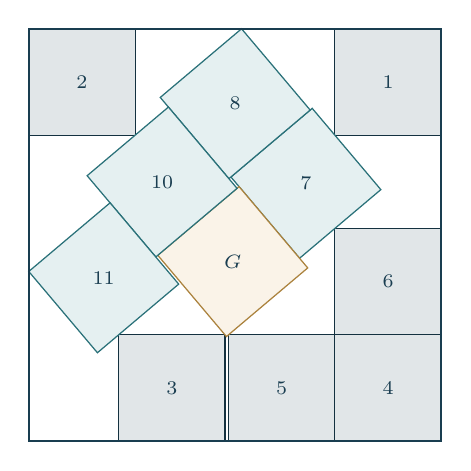
\begin{tikzpicture}[scale=1.35,font=\scriptsize]
\filldraw[fill=ink!13,draw=ink!80!black,line width=.45pt] (2.87924778,2.87924778) -- (3.88000000,2.87924778) -- (3.88000000,3.88000000) -- (2.87924778,3.88000000) -- cycle;
\node[text=ink] at (3.379624,3.379624) {$ 1 $};
\filldraw[fill=ink!13,draw=ink!80!black,line width=.45pt] (0.00000000,2.87924778) -- (1.00075222,2.87924778) -- (1.00075222,3.88000000) -- (0.00000000,3.88000000) -- cycle;
\node[text=ink] at (0.500376,3.379624) {$ 2 $};
\filldraw[fill=ink!13,draw=ink!80!black,line width=.45pt] (0.84516054,0.00000000) -- (1.84591276,0.00000000) -- (1.84591276,1.00075222) -- (0.84516054,1.00075222) -- cycle;
\node[text=ink] at (1.345537,0.500376) {$ 3 $};
\filldraw[fill=ink!13,draw=ink!80!black,line width=.45pt] (2.87924778,0.00000000) -- (3.88000000,0.00000000) -- (3.88000000,1.00075222) -- (2.87924778,1.00075222) -- cycle;
\node[text=ink] at (3.379624,0.500376) {$ 4 $};
\filldraw[fill=ink!13,draw=ink!80!black,line width=.45pt] (1.87849557,0.00000000) -- (2.87924778,0.00000000) -- (2.87924778,1.00075222) -- (1.87849557,1.00075222) -- cycle;
\node[text=ink] at (2.378872,0.500376) {$ 5 $};
\filldraw[fill=ink!13,draw=ink!80!black,line width=.45pt] (2.87924778,1.00075222) -- (3.88000000,1.00075222) -- (3.88000000,2.00150443) -- (2.87924778,2.00150443) -- cycle;
\node[text=ink] at (3.379624,1.501128) {$ 6 $};
\filldraw[fill=sea!13,draw=sea!80!black,line width=.45pt] (2.54735311,1.72121100) -- (3.31192728,2.36691321) -- (2.66622507,3.13148737) -- (1.90165090,2.48578517) -- cycle;
\node[text=ink] at (2.606789,2.426349) {$ 7 $};
\filldraw[fill=sea!13,draw=sea!80!black,line width=.45pt] (1.88263248,2.46972362) -- (2.64720664,3.11542583) -- (2.00150443,3.88000000) -- (1.23693027,3.23429779) -- cycle;
\node[text=ink] at (1.942068,3.174862) {$ 8 $};
\filldraw[fill=sand!13,draw=sand!80!black,line width=.45pt] (1.85947714,0.98469068) -- (2.62405131,1.63039288) -- (1.97834910,2.39496705) -- (1.21377493,1.74926484) -- cycle;
\node[text=ink] at (1.918913,1.689829) {$ G $};
\filldraw[fill=sea!13,draw=sea!80!black,line width=.45pt] (1.19475650,1.73320330) -- (1.95933067,2.37890551) -- (1.31362846,3.14347968) -- (0.54905429,2.49777747) -- cycle;
\node[text=ink] at (1.254192,2.438341) {$ 10 $};
\filldraw[fill=sea!13,draw=sea!80!black,line width=.45pt] (0.64570221,0.83230461) -- (1.41027638,1.47800682) -- (0.76457417,2.24258099) -- (0.00000000,1.59687878) -- cycle;
\node[text=ink] at (0.705138,1.537443) {$ 11 $};
\draw[ink,line width=.8pt] (0,0) rectangle (3.88,3.88);
\end{tikzpicture}\par\small The reference construction
\end{minipage}\hfill
\begin{minipage}[t]{.47\textwidth}\centering
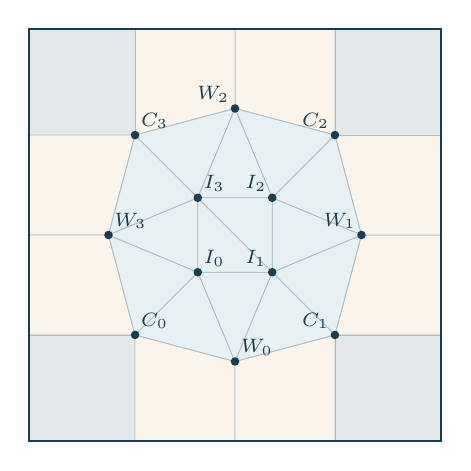
\begin{tikzpicture}[scale=1.35,font=\scriptsize]
\filldraw[fill=ink!12,draw=ink!35,line width=.3pt] (0.00000000,0.00000000) -- (1.00000000,0.00000000) -- (1.00000000,1.00000000) -- (0.00000000,1.00000000) -- cycle;
\filldraw[fill=sand!12,draw=ink!35,line width=.3pt] (1.00000000,0.00000000) -- (1.94000000,0.00000000) -- (1.94000000,0.75000000) -- (1.00000000,1.00000000) -- cycle;
\filldraw[fill=sand!12,draw=ink!35,line width=.3pt] (1.94000000,0.00000000) -- (2.88000000,0.00000000) -- (2.88000000,1.00000000) -- (1.94000000,0.75000000) -- cycle;
\filldraw[fill=ink!12,draw=ink!35,line width=.3pt] (3.88000000,0.00000000) -- (3.88000000,1.00000000) -- (2.88000000,1.00000000) -- (2.88000000,0.00000000) -- cycle;
\filldraw[fill=sand!12,draw=ink!35,line width=.3pt] (3.88000000,1.00000000) -- (3.88000000,1.94000000) -- (3.13000000,1.94000000) -- (2.88000000,1.00000000) -- cycle;
\filldraw[fill=sand!12,draw=ink!35,line width=.3pt] (3.88000000,1.94000000) -- (3.88000000,2.88000000) -- (2.88000000,2.88000000) -- (3.13000000,1.94000000) -- cycle;
\filldraw[fill=ink!12,draw=ink!35,line width=.3pt] (3.88000000,3.88000000) -- (2.88000000,3.88000000) -- (2.88000000,2.88000000) -- (3.88000000,2.88000000) -- cycle;
\filldraw[fill=sand!12,draw=ink!35,line width=.3pt] (2.88000000,3.88000000) -- (1.94000000,3.88000000) -- (1.94000000,3.13000000) -- (2.88000000,2.88000000) -- cycle;
\filldraw[fill=sand!12,draw=ink!35,line width=.3pt] (1.94000000,3.88000000) -- (1.00000000,3.88000000) -- (1.00000000,2.88000000) -- (1.94000000,3.13000000) -- cycle;
\filldraw[fill=ink!12,draw=ink!35,line width=.3pt] (0.00000000,3.88000000) -- (0.00000000,2.88000000) -- (1.00000000,2.88000000) -- (1.00000000,3.88000000) -- cycle;
\filldraw[fill=sand!12,draw=ink!35,line width=.3pt] (0.00000000,2.88000000) -- (0.00000000,1.94000000) -- (0.75000000,1.94000000) -- (1.00000000,2.88000000) -- cycle;
\filldraw[fill=sand!12,draw=ink!35,line width=.3pt] (0.00000000,1.94000000) -- (0.00000000,1.00000000) -- (1.00000000,1.00000000) -- (0.75000000,1.94000000) -- cycle;
\filldraw[fill=sea!12,draw=ink!35,line width=.3pt] (1.00000000,1.00000000) -- (1.94000000,0.75000000) -- (1.59000000,1.59000000) -- cycle;
\filldraw[fill=sea!12,draw=ink!35,line width=.3pt] (2.88000000,1.00000000) -- (3.13000000,1.94000000) -- (2.29000000,1.59000000) -- cycle;
\filldraw[fill=sea!12,draw=ink!35,line width=.3pt] (2.88000000,2.88000000) -- (1.94000000,3.13000000) -- (2.29000000,2.29000000) -- cycle;
\filldraw[fill=sea!12,draw=ink!35,line width=.3pt] (1.00000000,2.88000000) -- (0.75000000,1.94000000) -- (1.59000000,2.29000000) -- cycle;
\filldraw[fill=sea!12,draw=ink!35,line width=.3pt] (1.00000000,1.00000000) -- (1.59000000,1.59000000) -- (0.75000000,1.94000000) -- cycle;
\filldraw[fill=sea!12,draw=ink!35,line width=.3pt] (2.88000000,1.00000000) -- (2.29000000,1.59000000) -- (1.94000000,0.75000000) -- cycle;
\filldraw[fill=sea!12,draw=ink!35,line width=.3pt] (2.88000000,2.88000000) -- (2.29000000,2.29000000) -- (3.13000000,1.94000000) -- cycle;
\filldraw[fill=sea!12,draw=ink!35,line width=.3pt] (1.00000000,2.88000000) -- (1.59000000,2.29000000) -- (1.94000000,3.13000000) -- cycle;
\filldraw[fill=sea!12,draw=ink!35,line width=.3pt] (1.94000000,0.75000000) -- (2.29000000,1.59000000) -- (1.59000000,1.59000000) -- cycle;
\filldraw[fill=sea!12,draw=ink!35,line width=.3pt] (3.13000000,1.94000000) -- (2.29000000,2.29000000) -- (2.29000000,1.59000000) -- cycle;
\filldraw[fill=sea!12,draw=ink!35,line width=.3pt] (1.94000000,3.13000000) -- (1.59000000,2.29000000) -- (2.29000000,2.29000000) -- cycle;
\filldraw[fill=sea!12,draw=ink!35,line width=.3pt] (0.75000000,1.94000000) -- (1.59000000,1.59000000) -- (1.59000000,2.29000000) -- cycle;
\filldraw[fill=sea!12,draw=ink!35,line width=.3pt] (1.59000000,1.59000000) -- (2.29000000,1.59000000) -- (1.59000000,2.29000000) -- cycle;
\filldraw[fill=sea!12,draw=ink!35,line width=.3pt] (2.29000000,1.59000000) -- (2.29000000,2.29000000) -- (1.59000000,2.29000000) -- cycle;
\fill[ink] (1.0,1.0) circle (1.15pt) node[above right,inner sep=2pt] {$ C_0 $};
\fill[ink] (2.88,1.0) circle (1.15pt) node[above left,inner sep=2pt] {$ C_1 $};
\fill[ink] (2.88,2.88) circle (1.15pt) node[above left,inner sep=2pt] {$ C_2 $};
\fill[ink] (1.0,2.88) circle (1.15pt) node[above right,inner sep=2pt] {$ C_3 $};
\fill[ink] (1.94,0.75) circle (1.15pt) node[above right,inner sep=2pt] {$ W_0 $};
\fill[ink] (3.13,1.94) circle (1.15pt) node[above left,inner sep=2pt] {$ W_1 $};
\fill[ink] (1.94,3.13) circle (1.15pt) node[above left,inner sep=2pt] {$ W_2 $};
\fill[ink] (0.75,1.94) circle (1.15pt) node[above right,inner sep=2pt] {$ W_3 $};
\fill[ink] (1.59,1.59) circle (1.15pt) node[above right,inner sep=2pt] {$ I_0 $};
\fill[ink] (2.29,1.59) circle (1.15pt) node[above left,inner sep=2pt] {$ I_1 $};
\fill[ink] (2.29,2.29) circle (1.15pt) node[above left,inner sep=2pt] {$ I_2 $};
\fill[ink] (1.59,2.29) circle (1.15pt) node[above right,inner sep=2pt] {$ I_3 $};
\draw[ink,line width=.8pt] (0,0) rectangle (3.88,3.88);
\end{tikzpicture}\par\small Twelve markers and their cover
\end{minipage}
\caption{Both pictures use the normalized container of side $3.88$. The construction is scaled and half-turned; labels $1,\ldots,11$ follow Appendix~\ref{construction:exact}, with $G=9$ owning $I_0,I_1$. The right-hand partition consists of four corner rectangles, eight wall quadrilaterals, and fourteen triangles. Drawing coordinates are rounded; all proof comparisons are exact.}
\label{fig:packing-markers}\end{figure}
\begin{proposition}[Coarse global reduction]\label{input:global}
If eleven unit squares fit in a square of side less than $T$, there is an
improving representative whose six labeled squares, after the stated
normalization and half-turn, satisfy every hypothesis of
Theorem~\ref{thm:mixed-support}.
\end{proposition}
\begin{proof}
Choose the normalized side $a$ with
$a_*<a<A_+$ as in Section~\ref{hybrid:ownership}; the container has side
$S=97/25$ and returning to unit squares gives $L=S/a<T$.
The marker-cover and ownership lemmas give eight alternatives.
The exact certificates exclude cases $0$--$5$, and
Lemma~\ref{hybrid:opposite-inner} excludes case $7$. Thus only case $6$
remains, with common owner $G$ of $I_0,I_1$.

The symmetry restriction in Appendix~\ref{app:initial-corners} first gives
$0\le t_G\le\sqrt2-1$. The certified closed angle branches
$[0,5/24]$ and $[5/24,5/16]$ are excluded, leaving
$5/16<t_G\le\sqrt2-1$. A further closed-branch exclusion restricts
the $C_2$ owner's half-angle to
$[0,5/48)\cup(43/48,1]$. All branch endpoints are covered.
The coarse bounds and Proposition~\ref{prop:first-corner} permit the
first corner replacement. The separate obstruction exclusion and compact
separator argument in Appendix~\ref{app:second-corner-separator} permit
the second. Both replacements preserve the side length, ownership case
and angle of $G$; complete pose covers are regenerated afterward.

Iterate the necessary pose-cover rules, closed spatial exclusions and
virtual-support deductions in the supplement's dependency order.
Lemma~\ref{lem:rational-pose-bin} supplies valid enclosures on whole
angle intervals. Lemma~\ref{hybrid:boundary-neighborhood} and its
instantiation preserve actual centers through clipping, compatibility
pruning and rounding, including boundary contact. Each spatial exclusion
covers its closed contrary halfplane, so its surviving strict bound loses
no boundary case. The compact common-separator arguments in
Appendices~\ref{app:early-column} and \ref{app:early-bottom-row}, together
with the strip theorem, give the two label-specific virtual supports.

Every finite transition in this reduction has been replayed, with its
input and checker identities bound to the accepted parents. The selected
case-6 dependency graph has $119$ nodes and closes at the fifth prefix
of the final $N=384$ journal and its direct-support ending. Exact outward
comparison puts that prefix inside the three-decimal envelope
$\mathcal E$ of Section~\ref{sec:mixed-alignment}. The feature and sign
checks there establish the required corner, wall, bridge and two-normal
separator premises for every feasible packing in the entire envelope.
Scaling back to unit squares
and applying the half-turn therefore gives the asserted representative.
\end{proof}

\begin{theorem}[Eleven squares, computer-assisted]\label{thm:optimality}
The least side length of a square containing eleven closed unit squares
with pairwise disjoint interiors is $s(11)=T$.
\end{theorem}
\begin{proof}
The exact construction in Appendix~\ref{construction:exact} gives
$s(11)\le T$. If a smaller container were possible,
Proposition~\ref{input:global} would supply an improving representative
within the hypotheses of Theorem~\ref{thm:mixed-support}. Its conclusion
$L\ge T$ contradicts $L<T$.
\end{proof}

Only the first five rounds of the final $N=384$ journal are needed to
reach the displayed envelope. The seven remaining rounds of that journal,
all $32$ later refinement rounds, and the local-isolation endpoint are
not premises of the direct support proof. These savings concern the final
stage; the earlier global reductions remain part of the proof. The small
capture and local certificates are retained as supplementary checks.

\section{A finite ownership reduction}
\label{hybrid:ownership}

Fix
\[
 S=\frac{97}{25},\qquad A_- =\frac{4003}{4000},\qquad
 A_+=\frac{25019}{25000},\qquad a_* =\frac{S}{T}.
\]
The exact algebraic endpoint satisfies $A_-<a_*<A_+$.
If eleven unit squares fit in a container of side $L<T$, choose
\[
 a_*<a<\min\{A_+,S/L\}.
\]
Scaling by $a$ and enlarging the container gives eleven side-$a$ squares
in $[0,S]^2$. We shall exclude this possibility. The global reductions
use the slightly wider hypothesis $A_-<a<A_+$; the strict endpoints
provide slack in the rational pose enclosures.

A square \emph{owns} a marker when that marker belongs to its open
interior. A marker on a square boundary is not owned by that square.
Use the following twelve rational markers; all terminating decimals in
the table are exact.
\[
\begin{array}{c|cccc}
 &0&1&2&3\\ \hline
 C_j &(1,1)&(2.88,1)&(2.88,2.88)&(1,2.88)\\
 W_j &(1.94,.75)&(3.13,1.94)&(1.94,3.13)&(.75,1.94)\\
 I_j &(1.59,1.59)&(2.29,1.59)&(2.29,2.29)&(1.59,2.29)
\end{array}
\]

\begin{lemma}[Marker cover]
\label{hybrid:marker-cover}
Every square of side greater than $1$ contained in $[0,S]^2$ owns at
least one of the twelve markers.
\end{lemma}
\begin{proof}
Apply the rectangle, triangle, and wall-quadrilateral nonavoidance
lemmas of Stromquist~\cite{stromquist} to the position of the square's center. The required partition
consists of four $1$-by-$1$ corner rectangles, eight wall quadrilaterals,
and fourteen triangles. The wall quadrilaterals have width $47/50$
and inner endpoint heights $1$ and $3/4$.

The remaining octagon has cyclic boundary
$C_0,W_0,C_1,W_1,C_2,W_2,C_3,W_3$. Its triangles are the four rotations of
\[
 (C_0,W_0,I_0),\quad(C_0,I_0,W_3),\quad(W_0,I_1,I_0),
\]
together with $(I_0,I_1,I_3)$ and $(I_1,I_2,I_3)$.
Every triangle edge has length at most $1$. Centers on an edge cause no
gap: a chord through the center of a square has length at least its
side, so both endpoints of an edge of length at most $1$ cannot lie
outside a square of side greater than $1$.

For a wall quadrilateral, the nonavoidance condition is
\[
 \frac{\cos\theta}{1+\cos\theta}
 +\frac{1-(47/50)\cos\theta}{\sin\theta}>\frac34
 \qquad(0<\theta<\pi/2).
\]
Multiplying its difference by $100t$, where $t=\tan(\theta/2)$, gives
$3-25t+97t^2-50t^3$. On $0<t\le1/2$ this is at least
$3-25t+72t^2>0$, whose discriminant is $-239$.
On $1/2\le t<1$ it is at least $3-25t+47t^2$, increasing there and
equal to $9/4$ at $1/2$. The remaining hypotheses are
\[
 2\sqrt2-2<\frac{47}{50}<1,
 \qquad \left(\frac{47}{50}\right)^2+\left(\frac14\right)^2<1.
\]
The rational edge lengths, orientations, interior-edge cancellations,
and partition area are finite exact checks. The geometric nonavoidance
lemmas, rather than the area computation alone, give the asserted cover.
\end{proof}

\begin{proposition}[Eight ownership alternatives]
\label{hybrid:eight-cases}
Up to a symmetry of the container, every packing with $A_-<a<A_+$ has
one of the following ownership patterns. In an unused-marker case all
other markers have distinct singleton owners. In a pair case all other
markers have distinct singleton owners different from the pair owner.
\[
\begin{array}{c|l|l}
\text{case}&\text{exception}&\text{subsequent treatment}\\ \hline
0&C_0\text{ unused}&\text{finite exclusion}\\
1&W_0\text{ unused}&\text{finite exclusion}\\
2&I_0\text{ unused}&\text{finite exclusion}\\
3&C_0,W_0\text{ have one owner}&\text{finite exclusion}\\
4&C_0,I_0\text{ have one owner}&\text{finite exclusion}\\
5&W_0,I_0\text{ have one owner}&\text{finite exclusion}\\
6&I_0,I_1\text{ have one owner}&\text{normalization and coarse enclosure}\\
7&I_0,I_2\text{ have one owner}&\text{elementary exclusion}
\end{array}
\]
\end{proposition}
\begin{proof}
There are eleven disjoint nonempty ownership sets in a twelve-element
set. Either eleven markers are owned, one per square, or all twelve
are owned with exactly one double owner. Two markers owned by one square
have squared distance less than $2a^2<2A_+^2$.
Among the $66$ marker pairs, exactly $26$ pass this necessary diameter
test. Their five orbits under the eight square symmetries have sizes
$8,4,8,4,2$, with representatives given in cases $3$--$7$.
Unused markers form the three orbits $C$, $W$, and $I$.
These statements follow by applying the eight explicit permutations to
the rational marker coordinates.
\end{proof}

\begin{lemma}[Opposite inner markers]
\label{hybrid:opposite-inner}
Case $7$ is impossible.
\end{lemma}
\begin{proof}
Translate the inner marker square to vertices $(0,0),(d,0),(d,d),(0,d)$,
where $d=7/10$. Its proposed double owner contains $(0,0)$ and $(d,d)$
in its interior and does not contain the other two in its interior.
Choose perpendicular edge normals $u=(c,s)$ and $v=(-s,c)$ with
$c,s\ge0$ and $c^2+s^2=1$. Both excluded vertices have $u$-projections
between those of the owned vertices, hence lie strictly inside the
owner's $u$-strip. Their $v$-projections, $-ds$ and $dc$, must therefore
lie outside the open $v$-strip on opposite sides. That strip has width
at most $d(c+s)\le d\sqrt2<1$, contradicting $a>1$.
\end{proof}



\section{Two squares can cast the shadow of a straight row}
\label{sec:strip}
For a compact set $K$, write
\[
 h_K(n)=\max_{z\in K}n\cdot z,
 \qquad \ell_K(n)=\min_{z\in K}n\cdot z.
\]
Thus $h_K(n)\le\ell_R(n)$ says that a line perpendicular to $n$
separates $K$ from $R$, with $K$ on the lower side.  The following
lemma says that a pair of squares in a shallow strip casts at least as
large a shadow as a straight row, in every direction pointing into the
first quadrant.

\begin{theorem}[The strip lemma]
\label{thm:strip}
Let $P,Q$ be unit squares with disjoint interiors, both contained in
$\{x\ge0,\ 0\le y\le3/2\}$. Then, for every $r>0$,
\[
 h_{P\cup Q}(r,1)\ge 2r+1
   =h_{[0,2]\times[0,1]}(r,1).
\]
The same support comparison holds for every nonnegative direction,
including the coordinate directions by continuity.
\end{theorem}

The proof in Appendix~\ref{app:strip-proof} exhibits a point that would lie inside both squares if the support inequality failed.



\paragraph{What the lemma allows us to replace.}
It compares supports, not occupied regions. In particular, it does not
assert that the straight row lies in the original pair's union or convex
hull. Its useful consequence is instead the following precise rule.

\begin{lemma}[Transfer of a common separator]
\label{lem:virtual-transfer}
Suppose nonempty compact sets $E,P,Q$ satisfy
$h_E(n)\le\max\{h_P(n),h_Q(n)\}$ for every $n$ in a cone $\mathcal C$.
If a nonempty compact convex set $R$ has a common separator from $P$ and $Q$ with some
nonzero normal $n\in\mathcal C$, that is,
\[
 \max\{h_P(n),h_Q(n)\}\le\ell_R(n),
\]
then $R$ and $E$ have disjoint interiors.
\end{lemma}
\begin{proof}
The same line separates $E$ and $R$, since
$h_E(n)\le\max\{h_P(n),h_Q(n)\}\le\ell_R(n)$.
\end{proof}

Scaling and reflecting Theorem~\ref{thm:strip} yields the two virtual
rectangles needed in the packing. All squares below have side $a$ and
lie in $[0,S]^2$:
\begin{center}
\begin{tabular}{lll}
Pair confined to & Virtual rectangle $E$ & Allowed normals\\[2pt]
$x\ge S-3a/2$ & $[S-a,S]\times[0,2a]$ & $(-v,u)$, $u,v\ge0$\\
$y\le3a/2$ & $[S-2a,S]\times[0,a]$ & $(-v,u)$, $u,v\ge0$.
\end{tabular}
\end{center}
For any particular neighbour $R$, a common separator must still be
established. It is enough to establish it under the hypothesis that
the interiors of $R$ and $E$ meet: transfer then contradicts that hypothesis.
This is the role of the finite separating-axis checks in the existing
certificates. Pairwise nonoverlap with $P$ and $Q$, by itself, is not
sufficient.

\paragraph{One formula for both virtual obstacles.}
Write
\[
 E_{m,n}=[S-ma,S]\times[0,na],\qquad
 (m,n)\in\{(1,2),(2,1)\}.
\]
Let a neighbouring square have centre $C=(X,Y)$, side $a$, and unit edge
directions $e=(c,s)$ and $\nu=(-s,c)$, with $c,s\ge0$ and $c^2+s^2=1$.
Once the transfer lemma has proved
interior-disjointness from $E_{m,n}$, consider its upper-left corner
$p=(S-ma,na)$. If the independent pose bounds give
\[
 |e\cdot(p-C)|<a/2,\qquad \nu\cdot(p-C)<0,
\]
then $p$ cannot lie in the square's interior: every neighbourhood of this
corner meets the interior of $E_{m,n}$. It can therefore be excluded only
through its lower $\nu$-edge, so $\nu\cdot(p-C)\le-a/2$. Consequently
\begin{equation}\label{eq:virtual-unified}
 \boxed{\;-sX+cY\ge-sS+a\bigl(ms+nc+\tfrac12\bigr).\;}
\end{equation}
Thus the two virtual obstacles contribute the same elementary support
inequality, with $m,n$ interchanged. For the two named applications, the
global reduction supplies the pose bounds and common-separator premises;
the strip lemma itself supplies the support comparison.


\section{A mixed support inequality with independent angles}
\label{sec:mixed-alignment}

The common-angle hypothesis can be removed on a modest, explicitly stated
box. The argument below compares a scalar function at different angle
arguments. It does not move a packing or assume that the intermediate
angle assignments are feasible.

We use unit squares in $[0,L]^2$. Their centers are denoted by
$A,B,C,D,E,F$; $A,\ldots,E$ have angles
$\theta_A,\ldots,\theta_E$, and $F$ has angle $\phi$ near zero. Set
\[
 e_\theta=(\cos\theta,\sin\theta),\qquad
 n_\theta=(-\sin\theta,\cos\theta),\qquad
 w(\theta)=\cos\theta+\sin\theta,\qquad
 h(\theta)=\frac{1+w(\theta)}2.
\]
Here and throughout this section angles are measured in radians.
The fixed corner squares are $[0,1]^2$ and $[L-1,L]\times[0,1]$.
In the case-6 labeling, after undoing the normalized diagram's half-turn,
$A=I_2$, $B=W_2$, $C=G$, $D=I_3$, $E=W_3$, and $F=C_0$.

To specify the box with simple numbers, use normalized coordinates
$(X_Z,Y_Z)$ and a common normalized square side $a$, where
\[
 S=\frac{97}{25},\quad
 \frac{4003}{4000}\le a\le\frac{25019}{25000},\qquad
 Z=\left(\frac{S-X_Z}{a},\frac{S-Y_Z}{a}\right),\qquad L=\frac Sa.
\]
Put $\theta_0=2\arctan(73/200)$ and
$\epsilon_Z=\theta_Z-\theta_0$ for $Z=A,\ldots,E$.
All entries in the following table are exact terminating decimals.
\begin{center}
\begin{tabular}{c|c|c|c}
 & $X_Z$ & $Y_Z$ & $\epsilon_Z$ (or $\phi$ for $F$)\\ \hline
$A$&$[2.592,2.610]$&$[2.419,2.435]$&$[-.020,.027]$\\
$B$&$[1.931,1.946]$&$[3.169,3.178]$&$[-.034,.023]$\\
$C$&$[1.911,1.923]$&$[1.682,1.693]$&$[-.015,.004]$\\
$D$&$[1.248,1.261]$&$[2.429,2.442]$&$[-.038,.009]$\\
$E$&$[.700,.712]$&$[1.514,1.546]$&$[-.052,.027]$\\
$F$&$[1.336,1.352]$&$[.500,.510]$&$[-.014,.021]$
\end{tabular}
\end{center}
Call this six-square envelope $\mathcal E$. No angle equalities occur in
its definition.
The displayed box contains the freshly replayed pose cover after the first
five of the source's twelve final $N=384$ rounds. The exact containment
check and the support checks are bound to that fifth-prefix file by its
SHA256 digest. The last seven rounds are not premises of this section;
validity of the input to the five-round prefix is established by
Proposition~\ref{input:global}.

Here are the required geometric premises. The four corner or virtual
support gaps are
\[
\begin{aligned}
 g_{A0}&=e_{\theta_A}\cdot(A-(1,1))-\tfrac12,&
 g_{D0}&=n_{\theta_D}\cdot(D-(L-1,1))-\tfrac12,\\
 g_{Av}&=n_{\theta_A}\cdot((1,L-2)-A)-\tfrac12,&
 g_{Cv}&=n_{\theta_C}\cdot((2,L-1)-C)-\tfrac12.
\end{aligned}
\]
The wall and bridge gaps are
\[
\begin{aligned}
 g_{Bw}&=B_y-\tfrac12w(\theta_B),&
 g_{Ew}&=L-E_x-\tfrac12w(\theta_E),\\
 g_{Fw}&=L-F_y-\tfrac12(\cos\phi+|\sin\phi|),\\
 g_{CF}&=e_{\theta_C}\cdot(F-C)-h(\theta_C-\phi),&
 g_{EF}&=n_{\theta_E}\cdot(F-E)-h(\theta_E-\phi).
\end{aligned}
\]
All nine of these gaps are assumed nonnegative. The box ensures that
$0<\theta_C-\phi,\theta_E-\phi<\pi/2$, so the displayed support
formulas have the stated signs.

For five further pairs choose the oriented displacement $d$ and normal
family $v_\theta$ in this table:
\begin{center}
\begin{tabular}{c|c|c|c}
pair label&$(p,q)$&$d=q-p$&$v_\theta$\\ \hline
$AB$&$(B,A)$&$A-B$&$n_\theta$\\
$AC$&$(A,C)$&$C-A$&$e_\theta$\\
$BD$&$(B,D)$&$D-B$&$e_\theta$\\
$DE$&$(D,E)$&$E-D$&$e_\theta$\\
$CD$&$(D,C)$&$C-D$&$n_\theta$
\end{tabular}
\end{center}
The separator premise for each row is
\begin{equation}
 \max\{v_{\theta_p}\cdot d,v_{\theta_q}\cdot d\}
 \ \ge\ \frac{1+\cos(\theta_q-\theta_p)
                       +|\sin(\theta_q-\theta_p)|}{2}.
 \label{eq:mixed-family-premise}
\end{equation}
It permits either square's corresponding edge direction. It does not
prescribe which one separates, and does not require contact.

\begin{lemma}[Tree comparison for a scalar function]
\label{lem:mixed-tree}
Let a finite tree carry angle variables $\alpha_v$ and positive edge
weights $\beta_{vw}$. Fix its root angle and a differentiable function
$f$ of the other angles. Successively contract a leaf cluster into its
parent by varying all angle arguments in that cluster together until
they equal the parent's angle. Suppose that, along every such segment,
the absolute derivative of $f$ with respect to this common angle is
at most the weight of the contracted edge. Then
\[
 f(\text{all angles equal to the root})
 \ge f(\boldsymbol\alpha)-
       \sum_{vw}\beta_{vw}|\alpha_v-\alpha_w|.
\]
In particular the left side is nonnegative if the right side is.
\end{lemma}

\begin{proof}
Subtract the weighted sum of current tree differences from $f$.
During one contraction all these differences are constant except
the contracted edge's difference, which decreases to zero. The
derivative bound says the possible loss in $f$ is at most that decrease
times the edge weight. Thus the subtracted function cannot decrease.
Iterate until every tree difference is zero. These are evaluations
of a function; there is no requirement of geometric feasibility along
the intermediate paths.
\end{proof}

\begin{theorem}[Mixed support bound]
\label{thm:mixed-support}
Suppose the six squares have parameters in $\mathcal E$, the nine
corner, virtual, wall and bridge gaps above are nonnegative, and all
five separator premises \eqref{eq:mixed-family-premise} hold.
Then $L\ge T$.
\end{theorem}

This theorem isolates the analytic endpoint. Proposition~\ref{input:global}
supplies its hypotheses for every hypothetical improving packing. The
following proof establishes the stated implication throughout the closed
box; its finite checks do not separately replay the global reduction.

\begin{proof}
For a pair in the table, put
$m=(\theta_p+\theta_q)/2$, $\delta=(\theta_q-\theta_p)/2$, and
\[
 X=v_m\cdot d,\qquad Y=v_m^\perp\cdot d,\qquad
 g_{pq}=X-\cos\delta.
\]
The sign chosen for $v_m^\perp$ is immaterial. Taking the maximum in
\eqref{eq:mixed-family-premise} gives
\[
 X\cos\delta+|Y\sin\delta|
 \ge\cos\delta(\cos\delta+|\sin\delta|),
\]
therefore
\begin{equation}
 g_{pq}\ge(\cos\delta-|Y|)|\tan\delta|
 \ge\frac{\eta_{pq}}2|\theta_q-\theta_p|,
 \qquad
 \eta_{pq}=1-\frac{D_{pq}^2}{2}-B_{pq}>0.
 \label{eq:mixed-mismatch}
\end{equation}
Here $D_{pq}$ bounds $|\delta|$ and $B_{pq}$ bounds $|Y|$ throughout
$\mathcal E$. The last step uses $\cos\delta\ge1-\delta^2/2$ and
$|\tan\delta|\ge|\delta|$. Positivity of all five $\eta_{pq}$ is one
of the exact interval checks described below.

Let $u$ be the root in $(.36,.37)$ of
\[
 p(t)=5t^8-10t^7-2t^6+14t^5+12t^4-6t^3+2t^2+2t-1.
\]
Define the two support-chain functions
\[
 F_1(t)=\frac{4+6t}{1+2t-t^2},\qquad
 F_2(t)=\frac{4+8t-4t^2+20t^3+36t^4-4t^6+4t^7}
 {1+2t+2t^3+14t^4-2t^5-2t^7+t^8}.
\]
They satisfy $F_1(u)=F_2(u)=T$. Define the fixed algebraic number
\[
 \rho=\frac{-F_2'(u)}{F_1'(u)-F_2'(u)},\qquad
 \Psi(t)=\rho F_1(t)+(1-\rho)F_2(t).
\]
Exact polynomial checks give $0<\rho<1$, and both $F_1$ and $F_2$
are strictly convex on $[.34,.38]$. Thus $\Psi'(u)=0$ and
\begin{equation}
 \Psi(t)\ge\Psi(u)=T\qquad(.34\le t\le.38).
 \label{eq:mixed-scalar}
\end{equation}
Strict convexity is with respect to the half-angle parameter $t$;
no claim of convexity in all packing coordinates is needed.

Now anchor the weights at the actual angle of $C$:
\[
 \theta=\theta_C,\quad t=\tan(\theta/2),\quad
 c=\cos\theta,\quad s=\sin\theta,\quad
 Q=1+\frac{c^3}{s}+\frac{s}{c},\quad
 k_1=\frac{\rho}{c+s},\quad k_2=\frac{1-\rho}{Q}.
\]
The envelope implies $.34<t<.38$. Assign these positive weights:
\begin{center}
\begin{tabular}{c|c@{\qquad}c|c}
gap&weight&gap&weight\\ \hline
$g_{D0},g_{Cv},g_{CD}$&$k_1$
 &$g_{A0},g_{AC},g_{CF}$&$k_2s^2/c$\\
$g_{Av},g_{AB}$&$k_2c^2/s$
 &$g_{Bw}$&$k_2c/s$\\
$g_{Ew}$&$k_2$
 &$g_{Fw}$&$k_2s/c$\\
$g_{BD},g_{DE}$&$k_2c$
 &$g_{EF}$&$k_2s$
\end{tabular}
\end{center}
Write $\lambda_j$ for these weights and let
$\mathcal S=\sum_j\lambda_jg_j$ be the sum of all fourteen gaps.
The centers, $L$, the anchor $\theta_C$, and all weights will remain
fixed in the comparisons that follow.

If the five tilted angle arguments are all set to $\theta$ and
$\phi=0$, the coefficients of every center cancel. More explicitly,
\[
 g_{D0}+g_{Cv}+g_{CD}=(c+s)(L-F_1(t)),
\]
and the eleven other gaps, with their weights divided by $k_2$, sum
to $Q(L-F_2(t))$. These are identities for arbitrary centers.
Consequently the aligned value of the function is
\begin{equation}
 \mathcal S(\theta,\theta,\theta,\theta,\theta;0)
 =L-\Psi(t).
 \label{eq:mixed-stress-identity}
\end{equation}

First remove the bridge angle from the function. With the five other
angles at their actual values, put
\[
 \begin{aligned}
 A_0&=\lambda_{Fw}+\lambda_{CF}w(\theta_C)
                         +\lambda_{EF}w(\theta_E),\\
 V_0&=\lambda_{CF}(\cos\theta_C-\sin\theta_C)
           +\lambda_{EF}(\cos\theta_E-\sin\theta_E).
 \end{aligned}
\]
Only three gaps depend on $\phi$, and their difference is exactly
\[
 \mathcal S(\boldsymbol\theta;0)-\mathcal S(\boldsymbol\theta;\phi)
 =\frac12\left[A_0(\cos\phi-1)+\lambda_{Fw}|\sin\phi|
                                      -V_0\sin\phi\right].
\]
For $\phi\ne0$ this is
\[
 \frac{|\sin\phi|}{2}
 \left[\lambda_{Fw}-\operatorname{sgn}(\phi)V_0
                         -A_0\tan(|\phi|/2)\right]\ge0.
\]
The bracket is positive throughout $\mathcal E$, as certified below;
for $\phi=0$ the difference is zero.

Retain the four tree edges $AB,DE,BD,CD$ and choose the fixed rational constants
\[
 (\beta_{AB},\beta_{DE},\beta_{BD},\beta_{CD})
 =(1/10,1/20,7/100,1/10).
\]
\begin{center}
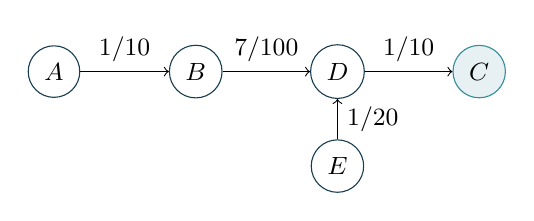
\begin{tikzpicture}[every node/.style={font=\small}]
\node[circle,draw=ink] (A) at (0,0) {$A$};
\node[circle,draw=ink] (B) at (1.8,0) {$B$};
\node[circle,draw=ink] (D) at (3.6,0) {$D$};
\node[circle,draw=sea,fill=sea!12] (C) at (5.4,0) {$C$};
\node[circle,draw=ink] (E) at (3.6,-1.2) {$E$};
\draw[->] (A) -- node[above] {$1/10$} (B);
\draw[->] (B) -- node[above] {$7/100$} (D);
\draw[->] (D) -- node[above] {$1/10$} (C);
\draw[->] (E) -- node[right] {$1/20$} (D);
\end{tikzpicture}
\end{center}
The arrows describe comparisons of angle arguments, not motions of squares.
The interval checks below establish
$0<\beta_e\le\lambda_e\eta_e/2$ uniformly over the entire envelope. Set
\[
 P(\boldsymbol\theta)=
 \beta_{AB}|\theta_A-\theta_B|
 +\beta_{DE}|\theta_D-\theta_E|
 +\beta_{BD}|\theta_B-\theta_D|
 +\beta_{CD}|\theta_C-\theta_D|.
\]
Equation~\eqref{eq:mixed-mismatch} and the other nonnegative gaps give
$\mathcal S(\boldsymbol\theta;\phi)\ge P(\boldsymbol\theta)$.
The unused $AC$ mismatch term is nonnegative and may be discarded.
The bridge comparison therefore gives
$\mathcal S(\boldsymbol\theta;0)\ge P(\boldsymbol\theta)$
at the actual angles.

We compare this function along four one-variable paths:
\begin{center}
\begin{tabular}{c|c|c|c}
step&angles moved together&starting value&ending value\\ \hline
1&$A$&$\theta_A$&$\theta_B$\\
2&$E$&$\theta_E$&$\theta_D$\\
3&$A,B$&$\theta_B$&$\theta_D$\\
4&$A,B,D,E$&$\theta_D$&$\theta_C$
\end{tabular}
\end{center}
The exact bounds below establish
\begin{equation}
 \left|\frac{d\mathcal S}{dq}\right|\le\beta_e
 \quad\hbox{along every segment in the table}.
 \label{eq:mixed-path-bound}
\end{equation}
Apply Lemma~\ref{lem:mixed-tree} to these four comparisons and use
\eqref{eq:mixed-stress-identity}:
\[
 L-\Psi(t)
 \ge \mathcal S(\boldsymbol\theta;0)-P(\boldsymbol\theta)\ge0.
\]
Combining this with \eqref{eq:mixed-scalar} proves $L\ge T$.
\end{proof}

\paragraph{Four interval checks.}
Appendix~\ref{app:mixed-intervals} specifies the rational interval
calculation. Four equal closed slices of $\theta_C-\theta_0\in[-.015,.004]$
suffice for the following uniform bounds:
\begin{center}
\begin{tabular}{c|c|c}
edge&$|d\mathcal S/dq|$ is at most&$\lambda_e\eta_e/2$ is at least\\ \hline
$AB$&$11/200$&$1/10$\\
$DE$&$9/200$&$1/20$\\
$BD$&$3/50$&$7/100$\\
$CD$&$49/500$&$1/10$
\end{tabular}
\end{center}
The bridge bracket exceeds $3/20$. These checks include every intermediate
angle on the four comparison paths. They also certify $\eta_{pq}>0$,
$.3127<\rho<.3128$, the root identities, and strict convexity of $F_1,F_2$.
All comparisons use exact rational bounds.


\paragraph{Why actual packings satisfy the selected support premises.}
For two squares, the separating-axis theorem supplies one of the eight
signed axes belonging to either square.  Test each such possibility by
projecting all four corners of the other square.  Over the displayed
closed boxes, rational Taylor bounds exclude 58 unwanted possibilities:
six for each of the five tilted pairs and seven for each of the four
corner or bridge pairs.  Every excluded possibility has a corner gap
strictly below zero; the smallest certified exclusion margin is greater
than $3/1000$ in the normalized coordinates.  The surviving axes are
exactly those displayed above and the unique axes of the four corner or
bridge inequalities.  Thus this finite check selects necessary supports
without selecting between the two possible owners of a tilted axis.

The six-square box also gives $\cos\theta_Q,\sin\theta_Q>0$ for every tilted
square, $\cos\phi>0$, and
$\cos(\theta_Q-\phi),\sin(\theta_Q-\phi)>0$ for $Q=C,E$.
The standard square support formula therefore gives the stated
inequalities, including the absolute value in the top-wall condition.
For each virtual obstacle, its relevant corner lies strictly inside the
square's transverse strip and strictly below its center in the normal
direction.  Avoiding the obstacle's interior consequently forces the
stated normal support.  All these sign and strip bounds are checked by
the same rational interval calculation.  Closed angle-bin endpoints and
all corner contacts are retained throughout.


The strict margins also determine the six-square block at equality; see Corollary~\ref{cor:mixed-block-rigidity}.

\section{Finite verification and its scope}\label{sec:verification}
The computation has two roles. The global part excludes the other marker
cases, justifies the two corner replacements, and confines the surviving
family. The endpoint part checks explicit support inequalities on the
resulting rational box. Its four interval slices bound four angular
derivatives and one bridge cost; polynomial sign tests establish the
convexity of the two scalar support functions. Neither a numerical
optimization result nor local rigidity substitutes for the global part.

The geometric rules are proved once in the appendices. Their finite
instances are checked with exact rational arithmetic and outward bounds.
The acceptance procedure then verifies the dependency links, branch
coverage, normalization interfaces and final enclosure. A successful
calculation on an unproved input is not an accepted global deduction.

\begin{center}\small
\begin{tabular}{@{}p{.28\textwidth}p{.64\textwidth}@{}}
\toprule
Component & Verification used in the argument\\\midrule
Foundation and construction & Arithmetic for the marker covers and
normalization bracket; containment of all $44$ construction vertices and
all $55$ pairwise separations.\\
Ownership cases $0$--$5$ & Complete exact exclusions from the initial
compulsory regions, with the stated symmetry restrictions. Case $7$ has
the elementary geometric exclusion.\\
Shortened case $0$ & A segment and a seven-vertex polygon give an ending
with $760$ promotions. Its required prefix and six new promotions are
freshly checked. The full replay command also rechecks the original
$794$-promotion exclusion.\\
Shortened cases $3,5$ & Respectively $62$ promotions in $11$ owner checks
and $170$ in $32$ checks, each ending at a shared interior point.\\
Surviving case $6$ & A closed $119$-node dependency graph joins the angle
exclusions, corner interfaces, spatial deductions, virtual supports and
selected endpoint. The nodes include the displayed mathematical rules.\\
Direct endpoint & The fifth of twelve final coarse-cover rounds lies
inside a three-decimal box. Exact feature and sign checks and four
interval slices prove the independent-angle support bound.\\
Alternative endpoint & Capture with at most $42$ rows and local isolation
with $41$ rows; supplementary and not needed for the direct argument.\\
Formal verification & No new Lean build or proof-kernel replay is claimed.\\
\bottomrule
\end{tabular}
\end{center}

The shortened mathematical argument and the verification schedule need
not have the same number of operations. A replay may check a longer
source prefix or a redundant certificate to validate an interface.
The recorded counts above specify which argument or computation they
measure; no claim of a minimum-size checker is made.

\paragraph{Observed verification and portable replay.}
All computational components used here were freshly replayed locally,
and their input-bound dependencies were composed to close both the six
ownership exclusions and the selected case-6 graph. The self-contained
small checks also passed. The portable full-run command has been prepared
and reviewed but has not yet been executed end to end; its reproduction
procedure is described in Section~\ref{sec:reproducibility}.

\paragraph{Boundary contact.}
A compulsory region may belong to a closed square without lying strictly
inside it; canonical corner vertices are examples. The proof keeps those
facts separate. A point in the interior of one square and the closed
square of another forces interior overlap by density, while an
intersection of two closed compulsory regions alone does not.
The relative-neighborhood invariant in
Appendix~\ref{sec:global-envelope} also justifies zero-area deletions
without assuming that feasible packings can be perturbed generically.

\paragraph{Trust model.}
This is an ordinary mathematical proof with computer-assisted finite
steps. It trusts the displayed geometric and analytic arguments, the cited
nonavoidance lemmas, the reviewed checker implementations and the CPython
runtime's exact integer and rational arithmetic. Accepted trigonometric
and algebraic comparisons use certified rational bounds. Numerical search
may propose a certificate; the replay checks its deductions afresh.
Hashes bind files and dependency identities, not geometric truth, and a
saved success flag is never a substitute for a required replay.

\paragraph{Formalization interface.}
The active closed-halfplane cover-tree theorems in the inspected Lean
repository \cite{formalized} give a useful future interface: split a closed
domain, retain a certified subdomain, or exclude it by checked inequalities,
while preserving points and segments. That development was inspected,
not rebuilt here. The present journals, variable side length, corner
replacements and virtual supports have not been translated into those
Lean theorems. The proof reported here uses the displayed polygon-cover
soundness argument instead.

\clearpage
\appendix


% New appendix fragment: root owns integration. No global replay is asserted here.
\section{Initial compulsory points and corner normalization}
\label{app:initial-corners}
Throughout this appendix the container is $[0,S]^2$, with
$S=97/25$ and $A_-<a<A_+$ as in Section~\ref{hybrid:ownership}.
The finite instances discussed below are checked in the supplement; their
geometric meaning is supplied by the following elementary rules.

\begin{lemma}[Moving one marker]\label{lem:moving-marker}
Suppose every side-$a$ square in the container contains a marker from
$M$ in its interior, and the same is true of
$(M\setminus\{m\})\cup\{q\}$. If a square owns $m$ and no other
marker of $M$, then it contains $q$ in its interior.
\end{lemma}
\begin{proof}
The square avoids every unchanged marker in its interior. Applying the
second cover leaves only $q$ as a possible interior marker.
\end{proof}
Apply this rule separately to finitely many proposed points and take their
convex hull. The resulting closed polygon lies strictly inside the owner.
The rule applies only to singleton owners; a square owning a pair of
original markers retains that pair as its initial compulsory set.

The initial inner and wall polygons are obtained in exactly this way.
For an inner singleton, move $I_0$ within the star with boundary
$C_0,W_0,I_1,I_3,W_3$, retaining the triangulation in
Lemma~\ref{hybrid:marker-cover}. The finite candidate points have coordinates
$(i/100,j/100)$, with $120\le i,j\le180$, lie on the inner side of all
five star edges, and are within distance $1$ of every star vertex.
The companion checks the triangulation for every vertex of their convex
hull. For a wall singleton the four alternatives replacing $W_0$ are
\[
 (97/50,33/50),\quad(97/50,41/50),\quad
 (48/25,37/50),\quad(49/25,37/50).
\]
Their adjacent wall-quadrilateral inequalities and triangulations are
checked by the same nonavoidance lemmas. Rotate these statements for the
other inner and wall markers.

Later regenerations also use seven alternatives for a singleton $C_0$:
\[
\begin{gathered}
 (489/500,A_-),\quad(981/1000,997/1000),\quad
 (493/500,991/1000),\quad(991/1000,493/500),\\
 (997/1000,981/1000),\quad(A_-,489/500),\quad(A_-,A_-).
\end{gathered}
\]
For an alternative $(x,y)$, the modified corner rectangle has sides
$x,y\le A_-<a$. Put $m=S/2$ and $b=3/4$.
The two adjacent wall quadrilaterals use parameters
$((m-x)/y,b/y)$ and $((m-y)/x,b/x)$ after scaling by $y$ and $x$,
respectively. In both scalings the physical square has side greater than
$1$. The finite arithmetic verifies the wall hypotheses, the fourteen
oriented triangles, their edge lengths and the partition identity.
Lemma~\ref{lem:moving-marker} then proves strict containment of all seven
points. These claims concern alternative marker covers, not approximate
positions of a proposed packing.

\paragraph{The symmetry restrictions used by the journals.}
Before any propagation, use the following reflection when necessary:
\begin{center}
\begin{tabular}{c|c|c}
case&owner whose angle is restricted&reflection\\ \hline
0&$I_0$&$x=y$\\
1&$W_2$&$x=S/2$\\
2&$I_2$&$x=y$\\
4&common owner of $C_0,I_0$&$x=y$\\
6&$G$, common owner of $I_0,I_1$&$x=S/2$\\
3,5&none&none
\end{tabular}
\end{center}
Each reflection preserves the stated exceptional ownership pattern and
fixes the designated owner, while permuting the other marker labels.
For the last row involving a common owner, it interchanges $I_0,I_1$.
For an edge-angle representative $\theta\in[0,\pi/2]$, reflection gives
the equivalent representative $\pi/2-\theta$. Choosing the smaller one
therefore ensures
\[
 0\le\theta\le\pi/4,\qquad
 t=\tan(\theta/2)\le\sqrt2-1<5/12,
\]
where the last inequality follows from $(17/12)^2>2$.
The rational bin restriction encloses this interval, including its
endpoints. No claim that later asymmetric compulsory hulls are invariant
under the reflection is needed: all deductions follow the chosen symmetry.

\begin{lemma}[Corner support]\label{lem:corner-support}
Let $P$ be a square of side $a$ contained in the quadrant $x,y\ge0$,
and set $E=[0,a]^2$. For every $n=(n_x,n_y)$ with $n_x,n_y\ge0$,
\[
 h_E(n)\le h_P(n).
\]
Consequently, if another square $R$ is separated from $P$ by
$h_P(n)\le\ell_R(n)$ with such a nonzero normal, then the same line
separates $E$ from $R$.
\end{lemma}
\begin{proof}
Translate $P$ toward both walls until its bounding box has lower corner
$(0,0)$, obtaining $P_0$. Choose edge vectors $(c,s),(-s,c)$ with
$c,s\ge0$ and $c^2+s^2=1$, and write $w=c+s$.
The center of $P_0$ is $(aw/2,aw/2)$. Since $1\le w\le\sqrt2$,
both absolute edge coordinates of $(a,a)$ relative to that center are at
most
\[
 a(1-w/2)w=\frac a2\bigl(1-(w-1)^2\bigr)\le a/2.
\]
Thus $(a,a)\in P_0$. Translating back adds a vector with nonnegative
coordinates, so
$h_P(n)\ge h_{P_0}(n)\ge n\cdot(a,a)=h_E(n)$.
The separation statement follows immediately. Reflections give the same
rule at any container corner.
\end{proof}

\paragraph{The finite interface for the first corner.}
In the surviving case, the two closed angle-branch exclusions give
$5/16<t_G\le\sqrt2-1$. The seven-round source
\path{corner-global-root-N96.json} starts from the initial compulsory
regions and covers the larger interval $5/16\le t_G\le5/12$.
Its complete center covers give the following coarse facts, checked by
\texttt{exact\_corner\_boxes.py}. These facts, together with that cover's
ancestry, are the finite premises of the next proposition.
Use inward coordinates $X=x$, $Y=S-y$ at the upper-left corner.
Let $P$ be the $C_3$ owner and $B$ the $I_3$ owner. Then
\begin{equation}\label{eq:first-corner-envelope}
\begin{array}{c|cc}
 &X\text{ of center}&Y\text{ of center}\\ \hline
P &[1/2,71/100]&[1/2,71/100]\\
B &[121/100,149/100]&[5/4,77/50].
\end{array}
\end{equation}
Writing the original edge angle of $B$ as $\theta_B\in[0,\pi/2]$,
we also have
\begin{equation}\label{eq:first-corner-tilt}
 c+s\ge13/10,\qquad c=\cos\theta_B,\quad s=\sin\theta_B.
\end{equation}
Every other square has original center satisfying
\begin{equation}\label{eq:first-corner-exterior}
 x\ge43/25\quad\hbox{or}\quad y\le54/25.
\end{equation}
These are outer bounds on all legal poses. The tilt bound is valid on
whole angle bins: $\cos\theta+\sin\theta$ is concave on $[0,\pi/2]$,
so checking both rational half-angle endpoints suffices.

\begin{proposition}[First corner replacement]\label{prop:first-corner}
Suppose a case-6 packing satisfies
\eqref{eq:first-corner-envelope}--\eqref{eq:first-corner-exterior}.
Replacing its $C_3$ owner by
\[
 E=[0,a]\times[S-a,S]
\]
while fixing the other ten squares gives another legal packing of the
same side length and ownership pattern. The angle of $G$ is unchanged.
\end{proposition}
\begin{proof}
The circumradius is $a/\sqrt2<71/100$, because
$A_+^2/2<(71/100)^2$. Each of the nine squares other than $P,B$
therefore lies wholly to the right of
$43/25-71/100=1.01>A_+$, or wholly below
$54/25+71/100=2.87<S-A_+$. They already miss $E$.

It remains to treat $B$. Work in the inward coordinates, in which the
replacement is $[0,a]^2$. Let $d$ be the displacement from the center
of $P$ to the center of $B$. The envelope gives
\[
 1/2\le d_x\le99/100,\qquad27/50\le d_y\le26/25.
\]
Since the original interiors are disjoint, a separating line has a unit
normal $n$ directed toward $B$. Each square contains its concentric disk
of radius $a/2$, so separation requires $n\cdot d\ge a>1$.
Normals with $n_x\ge0,n_y\le0$ give $n\cdot d\le99/100$;
those with both components nonpositive give $n\cdot d\le0$.

The only remaining unwanted normals are $n=(-e,f)$, where
$e>0$, $f\ge0$ and $e^2+f^2=1$. If $e\ge2/25$, then
\[
 n\cdot d\le-e/2+26/25\le1<a,
\]
which is impossible. If $0<e<2/25$, then $f>249/250$, since
$1-(2/25)^2>(249/250)^2$. In inward coordinates the edge vectors
of $B$ are $(c,-s)$ and $(s,c)$. Its centered support radius is
\[
\begin{aligned}
 r_B(n)&=\frac a2\bigl(|-ec-fs|+|-es+fc|\bigr)\\
 &\ge\frac a2\{f(c+s)+e(c-s)\}\\
 &>\frac a2\left\{\frac{249}{250}\frac{13}{10}-\frac2{25}\right\}
 >\frac{3a}{5}.
\end{aligned}
\]
Here $c-s\ge-1$ justifies the middle bound. The support radius of
$P$ is at least $a/2$, so separation would require
$n\cdot d>11a/10>11/10$. But $n\cdot d\le d_y\le26/25<11/10$.
Thus every separating normal points into the inward quadrant.
Lemma~\ref{lem:corner-support} transfers one such separator from $P$
to $E$, proving that $E$ also misses $B$ in its interior.

Containment in the container is automatic. The marker $C_3$ has inward
coordinates $(1,1)$ and lies strictly inside $E$ because $a>1$.
Every other marker has at least one inward coordinate greater than or
equal to $A_+$, as direct comparison with the marker table shows; none
is owned by $E$. All other owners remain fixed, and $P$ is distinct from
$G$. Hence ownership and the normalized angle restriction are preserved.
\end{proof}

After the replacement one must regenerate covers for the new packing;
one does not transport old center bounds through the replacement.
The marker-forcing statements remain globally valid and may be reapplied.
This is the first normalization interface used by
Proposition~\ref{hybrid:boundary-instantiation}. The second replacement
uses the upper-right reflection of Lemma~\ref{lem:corner-support} and the
separate obstruction exclusions in Appendix~\ref{app:second-corner-separator}.


% Integrate only after the fresh root/angle/corner replay queue has completed.
\paragraph{Angle reduction and the two corner replacements.}
Write $t_G=\tan(\theta_G/2)$ for the common marker owner's half-angle,
and $t_{C_2}=\tan(\theta_{C_2}/2)$ for the upper-right corner owner's
half-angle, in the normalized container $[0,S]^2$. The initial symmetry
choice gives $0\le t_G\le\sqrt2-1$. The angle exclusions use precisely
these closed branches:
\begin{center}
\begin{tabular}{c|c|c}
branch&common-owner interval&additional condition\\ \hline
lower&$[0,5/24]$&none\\
middle&$[5/24,5/16]$&none\\
corner&$[5/16,5/12]$&$t_{C_2}\in[5/48,43/48]$
\end{tabular}
\end{center}
Since $\sqrt2-1<5/12$, their complement gives
\[
 \frac5{16}<t_G\le\sqrt2-1,
 \qquad t_{C_2}\in[0,5/48)\cup(43/48,1].
\]
Every endpoint in the excluded branches is included in a checked closed
angle bin. The strict inequalities in the surviving intervals are
therefore consequences of closed exclusions, not endpoint conventions.
Subtracting $\pi/2$ from the near-vertical corner angle gives the single
lifted half-angle interval $(-5/91,5/48)$, using
$(43/48-1)/(43/48+1)=-5/91$.

The corner steps then make two existence-preserving replacements:
\begin{center}
\begin{tabular}{c|c|p{.49\linewidth}}
step&replacement square&reason replacement preserves nonoverlap\\ \hline
first&$[0,a]\times[S-a,S]$&
Coarse bounds separate nine other squares directly. The only possible
neighbor has an inward separating normal, so corner support domination
applies.\\
second&$[S-a,S]^2$&
A separate obstruction branch excludes interference by the top-wall
owner. Exact edge-direction exclusions force inward separation from
every remaining possible obstruction.
\end{tabular}
\end{center}
Both replacements keep the side length, marker assignment and common
owner's angle. The other nine squares remain fixed after both steps.
Thus the previously established compulsory-hull statements apply again
to the new packing. The initial hulls of each replaced corner also lie
inside its canonical corner square directly. Fresh midpoint-angle covers
are regenerated for the resulting centers; this is where the boundary
invariant is reestablished. Neither replacement asserts uniqueness of the
original packing.


\section{One principle for the global reduction}
\label{sec:global-envelope}

The global argument can be organized around a simple distinction: where a
square \emph{might be}, and what it \emph{must contain}.  This section proves
the general deduction rules. Their finite instances and dependency links
are verified by the accepted global certificate. A sound local operation
and a complete ancestry are separate parts of that verification.

Fix the small-square side $a>0$.  For a pose $p=(z,\theta)$, put
\[
 Q(p)=z+R_\theta[-a/2,a/2]^2.
\]
Fix a branch of the argument, with explicitly stated assumptions, and let
$\mathcal F$ be the set of actual labelled packings satisfying them.
For label $i$, keep a set $D_i$ of possible poses, a compact polygon $K_i$,
and an optional compact region $I_i$ with a separate strict-containment proof.
The invariant is that, for every $P\in\mathcal F$,
\begin{equation}
 p_i(P)\in D_i,
 \qquad K_i\subset Q(p_i(P)),
 \qquad I_i\subset\operatorname{int}Q(p_i(P)).
 \tag{G}\label{eq:global-invariant}
\end{equation}
Empty $K_i$ and $I_i$ are allowed.  The domains $D_i$ are outer bounds;
the \emph{compulsory regions} $K_i$ give closed containment, whereas $I_i$
records strict interior containment.  This distinction matters after a
corner replacement: the canonical square's vertices on the container wall
belong to $K_i$, but cannot belong to $I_i$.
The domains may contain spurious poses, and no independence of the
eleven poses is asserted.

\begin{lemma}[Making compulsory regions]\label{lem:compulsory-hulls}
If a compact polygon $K$ lies in $Q(p)$ for every $p\in D_i$, it may be
added to $K_i$.  If the containment is strict, it may also be added to $I_i$.
The convex hull of finitely many closed compulsory polygons for one label
is closed compulsory; the convex hull of finitely many strict compulsory
polygons for one label is strict compulsory.
\end{lemma}

\begin{proof}
The first assertions follow by substituting the actual pose in (G).
Both a closed square and its interior are convex, so the respective set
contains every convex combination of the finitely many polygon vertices.
\end{proof}

This rule combines points owned by \emph{one} square.  Points owned by
different squares cannot be combined in this way.  Nor can one freely
take closures of infinite unions of strict inner sets.

\begin{lemma}[Compulsory rectangle]\label{lem:compulsory-rectangle}
If a square $Q$ of side $b>0$ is contained in
$[L,R]\times[B,H]$, where $R-L\leq2b$ and $H-B\leq2b$, then
\[
 [R-b,L+b]\times[H-b,B+b]\subseteq Q.
\]
The rectangle is allowed to degenerate to a segment or point.
\end{lemma}

\begin{proof}
Choose unit edge vectors $(c,s),(-s,c)$ with $c,s\geq0$, and put $w=c+s$.
The center $(X,Y)$ satisfies
\[
 L+bw/2\leq X\leq R-bw/2,\qquad
 B+bw/2\leq Y\leq H-bw/2.
\]
For $(x,y)$ in the claimed rectangle,
$|x-X|,|y-Y|\leq b(1-w/2)$.  Each absolute edge coordinate is at most
\[
 bw(1-w/2)=\frac b2\bigl(1-(w-1)^2\bigr)\leq\frac b2,
\]
which is exactly the condition for membership in $Q$.
\end{proof}

This is a \emph{closed} containment statement.  The interior of a
full-dimensional core rectangle lies strictly inside $Q$, but its boundary
need not.  To obtain an entire closed compulsory rectangle for an actual
square of side $a$, choose $0<A_-<a$, enclose its concentric subsquare of
side $A_-$ in a proved common bounding box, and apply the lemma with
$b=A_-$.  The whole resulting core lies in the subsquare and hence strictly
inside the actual square, including when the core is a segment or point.

\begin{lemma}[Convexifying a center cover]\label{lem:convex-center-cover}
For a nonempty center set $E$ and any fixed convex set $Q_0$,
\[
 \bigcap_{z\in E}(z+Q_0)
 =\bigcap_{z\in\operatorname{conv}E}(z+Q_0).
\]
\end{lemma}
\begin{proof}
One inclusion follows from $E\subseteq\operatorname{conv}E$.
For the other, let $x$ lie in every $z+Q_0$ for $z\in E$.
If $y=\sum_k\lambda_k z_k$ is a finite convex combination from $E$, then
$x-y=\sum_k\lambda_k(x-z_k)\in Q_0$ by convexity.
\end{proof}
Thus, for a fixed reference core in an angle interval, replacing its
center cover by its convex hull loses no common-core information.
This does not assert that all the added center poses are feasible.

\begin{lemma}[Necessary restrictions and collision]\label{lem:pose-restrictions}
The following operations preserve (G).
\begin{enumerate}
 \item Delete poses violating any proved necessary condition for label $i$,
 including containment in the actual container,
 $K_i\subset Q(p)$, or $I_i\subset\operatorname{int}Q(p)$.
 \item Delete a pose $p\in D_i$ if
 $\operatorname{int}Q(p)\cap K_j\ne\varnothing$ for some $j\ne i$.
 \item Replace $D_i$ by any $D'_i$ containing every pose in $D_i$ that has
 not been proved impossible.  In particular, enlarging a domain is safe,
 though it can weaken later deductions.
\end{enumerate}
\end{lemma}

\begin{proof}
An actual pose satisfies every necessary condition.  In the second
operation, let $x\in\operatorname{int}Q(p_i(P))\cap K_j$.  Although $x$
may lie on the boundary of $Q(p_j(P))$, its interior is dense in that closed
square.  A sufficiently small neighborhood of $x$ lies inside
$\operatorname{int}Q(p_i(P))$ and contains a point of
$\operatorname{int}Q(p_j(P))$, contrary to the packing condition.
The third operation
retains each actual pose by construction.  Existing compulsory regions
remain valid because they are statements about actual packings.
\end{proof}

The collision test has a useful uniform form.  Let $I$ be an angle interval,
and suppose the compact set $A\subset\operatorname{int}Q(0,\theta)$ for
every $\theta\in I$.
For a different owner's compulsory region $K_j$, every center in
\[
 K_j+(-A)=\{k-u:k\in K_j,\ u\in A\}
\]
is forbidden throughout that angle interval.  For $z=k-u$, the point
$k=z+u$ belongs to the foreign closed square and to the interior of the
square being tested.  The density argument in the proof above gives an
interior overlap.  Thus a \emph{closed} forbidden polygon may be deleted:
strict containment of the reference core $A$ suffices, even when $K_j$
contains boundary points.  A genuine center lies outside this compact
forbidden set and therefore has positive distance from it.  Ordinary
boundary contact between the two actual squares remains permitted.

\begin{lemma}[Compatibility pruning]\label{lem:arc-consistency}
For $i\ne j$, let $C_{ij}(p,q)$ be any relation satisfied by all actual
pose pairs in $\mathcal F$.  Replace $D_i$ by any superset of
\[
 \{p\in D_i:\text{for every }j\ne i\text{ there exists }q\in D_j
                   \text{ with }C_{ij}(p,q)\}.
\]
The invariant is preserved.  This is usually called arc consistency.
\end{lemma}

\begin{proof}
For an actual pose $p_i(P)$, the witness for label $j$ is $p_j(P)$.
All these witnesses belong to their current domains by (G).
\end{proof}

For example, $C_{ij}$ may mean that the two square interiors are disjoint,
or it may be a weaker, easier necessary condition.  A pose can therefore
be removed when it collides with \emph{every} pose in a complete partner
domain.  Testing only selected partner poses is insufficient.  Pairwise
compatibility is a necessary condition; surviving it does not establish
that the eleven poses can occur together.

\paragraph{Virtual obstacles have a different logical role.}
A virtual obstacle $V_i$ for label $i$ means that a separate theorem proves
\[
 \operatorname{int}Q(p_i(P))\cap\operatorname{int}V_i=\varnothing
 \qquad(P\in\mathcal F).
\]
It is a necessary restriction on that label, not an assertion that an
actual square occupies $V_i$.  Lemma~\ref{lem:pose-restrictions} permits deleting any pose violating
this restriction.  If $J\subset\operatorname{int}V_i$ and $A$ is a strict
core for an angle interval as above, then $J+(-A)$ is a forbidden center
set for label $i$.
More generally, a strip theorem may supply a necessary separation
inequality rather than a virtual region; that inequality can be used
directly under Lemma~\ref{lem:pose-restrictions}.
Such a restriction applies to another label only with its own justification.
Intersecting two virtual obstacles is not a packing contradiction.

\paragraph{Branching, contradictions, and capture.}
These deductions may be iterated.  A branch is impossible if some $D_i$
is empty, if $I_i\cap K_j\ne\varnothing$ for distinct labels, or if
$K_i\cap\operatorname{int}V_i\ne\varnothing$.  The latter two conclusions
follow from (G) and the density argument above.  An intersection
$K_i\cap K_j\ne\varnothing$ alone is insufficient, since it may represent
legal boundary contact.  To replace one branch by several, their assumptions
must cover every actual packing in the parent branch; overlap is harmless.
Likewise, a polygonal update must cover the old domain by justified
forbidden regions and retained regions.  Edges, isolated points, and
equality cases must be included.

If every terminal branch is either impossible or has
$D_1\times\cdots\times D_{11}$ inside a specified local neighborhood
(in the required labels and coordinates), induction proves capture into
that neighborhood for the original branch.  This is the general soundness
argument for a finite elimination certificate.  Its premises include the
initial cover and every restriction, inner-region promotion, branch cover,
and final inclusion.  They cannot be replaced by a count of terminal cases
or an assertion that a search succeeded.

In the fixed-container normalization used here, the application starts
with a hypothetical improvement $a>a_*$, where $a_*$ is the known
construction's small-square side. The ownership classification,
side-preserving corner replacements and complete coarse enclosure are
established in the respective parts of Proposition~\ref{input:global}.
The general rules above justify their composition. No classification of
every endpoint packing or full eleven-square uniqueness is asserted.


\begin{lemma}[A rational certificate for an entire angle interval]
\label{lem:rational-pose-bin}
Let $0<A_-<a<A_+$, let $N\ge1$ and $0\le k<N$ be integers,
choose $\theta\in[0,\pi/2]$, and suppose
\[
 \tan(\theta/2)\in[k/N,(k+1)/N]\subseteq[0,1].
\]
Put $t_k=(2k+1)/(2N)$,
\[
 c_k=\frac{1-t_k^2}{1+t_k^2},\qquad
 s_k=\frac{2t_k}{1+t_k^2},\qquad
 q=1+\frac1N,\quad H=\frac{A_+q}{2},\quad h=\frac{A_-}{2q}.
\]
In the orthonormal frame with axes $(c_k,s_k),(-s_k,c_k)$,
the actual square with center $z$ contains $z+[-h,h]^2$ strictly and
is strictly contained in $z+(-H,H)^2$.
If $E$ is a nonempty center polygon with rational vertices in this frame and
\[
 x_-=\min_E x,\quad x_+=\max_E x,\quad
 y_-=\min_E y,\quad y_+=\max_E y,
\]
then each point in
\[
 [x_+-h,x_-+h]\times[y_+-h,y_-+h]
\]
is strictly inside every actual square whose center lies in $E$ and
whose angle lies in the stated interval. An interval with reversed
endpoints denotes the empty set.
\end{lemma}
\begin{proof}
Since $|(2\arctan t)'|\le2$, the actual angle differs from
$2\arctan t_k$ by at most $1/N$. The sum of the absolute sine and
cosine of this difference is at most $1+1/N=q$. Rotating the actual
square to the midpoint frame therefore gives coordinate half-width
at most $aq/2<H$. Conversely, the midpoint square of half-side $h$
has coordinates of absolute value at most $hq=A_-/2<a/2$ in the
actual square's frame. This proves both strict inclusions. Intersecting
$z+[-h,h]^2$ over $z\in E$ gives exactly the displayed rectangle.
The extrema $x_\pm,y_\pm$ occur at vertices of $E$ and are rational.
\end{proof}

Thus a forced-point promotion is a finite comparison with polygon
extrema, valid for every center and every angle in a closed interval.
A foreign compulsory hull $K_j$, expressed in the same frame, forbids the closed center region
$K_j+[-h,h]^2$ in this midpoint frame. Polygon clipping, convex hulls,
and these comparisons use rational arithmetic. Angle subdivision,
compatibility deletion and the boundary invariant justify their repeated
use; they are not tests at finitely many sampled orientations.


\begin{lemma}[Preservation of boundary centers]
\label{hybrid:boundary-neighborhood}
Fix a legal packing satisfying $A_-<a<A_+$ and the current branch
hypotheses. For owner $i$, let $z_i$ be its actual center. Let $C_i$ be
$\mathbb R^2$, except that the owner of a nontrivial spatial branch has
the branch's single closed halfplane as $C_i$. An identity branch such
as $0\le1$ leaves $C_i=\mathbb R^2$. For each tracked angle bin $J$ containing
the owner's actual angle, let $U_{i,J}$ be the union of its finitely many
closed convex center polygons, expressed in physical coordinates.
Assume that $z_i\in C_i$ and that at least one tracked bin contains each
actual angle.
The latter angle-cover obligation is separate from the center-domain
argument below.

Suppose initially, for some $\varepsilon>0$,
\begin{equation}
 B(z_i,\varepsilon)\cap C_i\subseteq U_{i,J}.
 \label{hybrid:relative-neighborhood}
\end{equation}
Then this property, with possibly smaller $\varepsilon$, is preserved by
finite compositions of the following operations:
\begin{enumerate}
\item clipping by finitely many closed halfplanes strict at $z_i$, or
by a union of such halfplanes of which at least one is strict at $z_i$;
\item subtraction of closed forbidden sets not containing $z_i$;
\item deletion of whole pose components by an incompatibility rule
that never rejects a pair of components containing the two actual
centers in bins containing their actual angles;
\item convexification, strict outward polygon rounding, and rotation of
coordinates during an angle subdivision covering the actual angle.
\end{enumerate}
Zero-area pieces may be discarded after these operations. A single closed
spatial branch halfplane may also be introduced from an ordinary
neighborhood in the unbranched cover.
\end{lemma}

\begin{proof}
A finite collection of strict halfplane inequalities holds in a ball
about $z_i$. The same is true of one strict member of a union. A closed
forbidden set missing $z_i$ misses a sufficiently small ball about it.
Intersect these balls with the neighborhood in
\eqref{hybrid:relative-neighborhood}.

To justify discarding zero-area pieces, take any point $x$ of a smaller
relative neighborhood. It is a limit of points in the interior of $C_i$
avoiding the finitely many polygon edges and clipping lines. Such points
belong to two-dimensional retained pieces. A subsequence belongs to one
of the finitely many closed retained pieces, so its limit $x$ belongs to
that piece as well. The same argument introduces a closed branch
halfplane, since a nontrivial halfplane is the closure of its interior.
This is an argument about the union of components, rather than a claim
that each individual component meeting the branch boundary survives.

A sound incompatibility deletion cannot remove a pose polygon containing
the actual center in an actual-angle bin: the actual partner pose supplies
a compatible witness. This observation inducts through the finite
arc-consistency procedure. Every deleted closed polygon missing $z_i$
has positive distance from it; finitely many such deletions therefore
preserve a smaller relative neighborhood.

Convexification and enlargement cannot remove points. Strict outward
rounding in fact restores an ordinary neighborhood whenever a retained
polygon contains $z_i$: each new support bound is strictly larger than
its old maximum, and the auxiliary universal center box contains $z_i$
strictly. Rotations are homeomorphisms, and the child angle bins cover
their parent. These observations complete the induction.
\end{proof}

\begin{proposition}[Instantiation for the surviving case]
\label{hybrid:boundary-instantiation}
The regenerated covers after each of the two corner normalizations
establish \eqref{hybrid:relative-neighborhood} for the resulting packing.
The subsequent center-domain operations preserve it, including all ten
one-halfplane spatial exclusions, both virtual support cuts, and the final
actual-edge pruning. It uses the ownership, normalization and support
theorems and the exact acceptance of each finite certificate, supplied by
the respective parents in the global reduction.
\end{proposition}

\begin{proof}
Each corner replacement changes the packing. Fix the resulting canonical
packing and reapply the globally valid compulsory-hull statements, whose
ownership and common-owner angle hypotheses are preserved. The source
then regenerates its covers. This establishes a new invariant at the new
centers; it does not transport neighborhoods through a corner replacement.

For a bin of half-angle width $1/N$, set
\[
 q=1+\frac1N,\qquad H=\frac{A_+q}{2},\qquad
 h=\frac{A_-}{2q}.
\]
The actual closed square lies strictly inside the midpoint square of
half-side $H$, while the closed midpoint square of half-side $h$ lies
strictly inside the actual square. The first strict inclusion follows
from $a<A_+$ and the second from $a>A_-$. Thus own-hull cuts are strict
even when a compulsory point belongs only to the closed owner square.
Relaxed wall cuts using $A_-$ are also strict. They give the initial
ordinary center neighborhoods.

The canonical corner centers have coordinates $a/2$ or $S-a/2$.
Their imposed coordinate rectangles use the endpoints $A_-/2,A_+/2$
or $S-A_+/2,S-A_-/2$, so their constraints are strict. The source keeps
these rectangles rather than imposing a lower-dimensional equality of
center coordinates. Obstruction conditioning is strict too: an actual
intersection point lies in the enlarged obstacle, and the actual square
lies strictly inside its outer midpoint square. The center consequently
lies in the interior of their Minkowski sum.

For a closed foreign compulsory hull $K_j\subset Q_j$, membership of
$z_i$ in $K_j-A$, where $z_i+A\subset\operatorname{int}Q_i$, would give
$x\in\operatorname{int}Q_i\cap Q_j$. Moving $x$ slightly toward the
center of $Q_j$ gives a point in both interiors, a contradiction.
Hence every closed foreign-hull forbidden set misses $z_i$.
Similarly, the universal inner-core collision regions are closed and
forbidden: even contact of the two closed cores gives intersection of
the actual open square interiors.

The actual-edge forbidden regions use the threshold
\[
 \frac{A_-}{2}(1+g)-\frac3{N^2},
\]
where $g$ is the lower bound for the relative-angle support factor.
Closed membership in the endpoint strips bounds every actual separating
projection by $A_-(1+g)/2$ after the interpolation allowance. The actual
support sum is at least $a(1+g)/2$, which is strictly larger. No actual
edge can separate the pair, again a contradiction. The forbidden regions
therefore miss $z_i$ as closed sets, including their boundaries.
Here the interpolation allowance follows from
$|z_i-z_j|\le S\sqrt2<6$ and angular bin width at most $2/N$:
the linear interpolation error is at most $6(2/N)^2/8=3/N^2$.

Each spatial branch imposes just one nontrivial closed halfplane, or the
identity $0\le1$. Every subsequently reapplied global spatial bound is
strict because its opposite closed branch has been excluded. Outward
rounding uses $(\lceil D b\rceil+1)/D>b$ for each support maximum $b$;
the enclosing box $[-8,8]^2$ contains actual midpoint-frame centers
strictly. Angle refinement preserves these properties.

For either virtual support inequality, replacing $a$ by $A_-$ makes
the necessary inequality strict. More explicitly, the two functions
whose endpoint upper bound is $1/(2N^2)$ are
\[
 f_{\rm col}(\theta)=
 \sin\theta(X-S+A_-)-\cos\theta(Y-2A_-)+A_-/2,
\qquad
 f_{\rm row}(\theta)=
 \sin\theta(X-S+2A_-)-\cos\theta(Y-A_-)+A_-/2.
\]
At the actual angle their values are at most, respectively,
$-(a-A_-)(\sin\theta+2\cos\theta+1/2)$ and
$-(a-A_-)(2\sin\theta+\cos\theta+1/2)$, and hence are negative.
The certified coordinate bounds give $|f''|<1$, so the linear
interpolant of the endpoint values is strictly below $1/(2N^2)$ at
the actual angle. At least one endpoint value is therefore strictly
below this bound. Thus the actual center is strictly in at least one
of the two endpoint halfplanes. The algorithm takes their union
before convexification.
The column's repeated coarse box
$[2.4,2.7]\times[2.3,2.6]$ contains the preceding exact source cover with
positive margins on all four sides. The bottom-row coarse box
$[1.90,1.94]\times[1.67,1.705]$ consists of four independently proved
strict spatial inequalities. In particular the relaxed source cover
may touch $X=1.90$, while an actual packing satisfies $X>1.90$.

All remaining steps are the operations of
Lemma~\ref{hybrid:boundary-neighborhood}. The approximating center
points used in that lemma are points of conservative domains; no nearby
legal packing and no generic-position hypothesis are asserted.
\end{proof}

\paragraph{Finite checks and replay scope.}
The static boundary audit of the full inherited-source graph records
$145$ nodes, $91$ occurrences of a spatial branch and $11$ distinct cuts:
the identity and the ten single halfplanes. Its $36$ cumulative
spatial-bound records are strict, and its $33$ journal rounding
denominators are positive. The smallest of the four freshly checked
column-box margins exceeds $0.048$. These are finite interfaces for the
boundary argument. The selected proof uses a different, $119$-node
acceptance graph, whose required geometric transitions are separately
replayed from accepted parents. Historical hashed inputs remain immutable.


\section{Verifying the four interval bounds}\label{app:mixed-intervals}
\paragraph{The small exact certificate.}
Here are details sufficient to specify the interval verification of the
inequalities used in the proof. Split the anchor-offset interval
$[-.015,.004]$ into four equal closed intervals. For each interval, enclose
all displayed weights using rational interval arithmetic, and choose
lower bounds for $\lambda_e\eta_e/2$ using the positive
rational $\eta_e$ from \eqref{eq:mixed-mismatch}.
The chosen fixed $\beta_e$ are no greater than any of the corresponding
four lower bounds. The centers use the rectangles obtained by
reflecting the displayed coordinate intervals about $S$ and dividing by
$[4003/4000,25019/25000]$. This enlargement loses correlations but preserves
containment. Bound each moving angle over the whole closed interval
between its two possible endpoint ranges, including the current anchor
interval in the fourth step.

For clarity, all derivatives being bounded can be recovered from the
gap definitions. If $d=q-p$ is the fixed displacement of a pair and
$g_{pq}=v_m\cdot d-\cos\delta$, then the derivative when just the
$p$ angle moves is
\[
 \tfrac12v_m'\cdot d-\tfrac12\sin\delta,
\]
and when just the $q$ angle moves it is
$\tfrac12v_m'\cdot d+\tfrac12\sin\delta$.
When both angles belong to a previously aligned moving cluster,
$\delta=0$ and the derivative is $v_q'\cdot d$, with $q$ now denoting
the common angle parameter. Together with direct differentiation of the
nine other gaps, these formulas give precisely the four derivatives
in \eqref{eq:mixed-path-bound}. The non-tree $AC$ gap must still be
included when one of its angles moves.

One convenient enclosure for an angular projection is as follows. If
$f(q)=v_q\cdot z$ and $z$ ranges over a rectangle, evaluate $f$ at each
rectangle vertex and at the two angle endpoints. Enlarge the resulting
interval by
\[
 \frac{(\max|z_x|+\max|z_y|)(q_+-q_-)^2}{8}.
\]
The linear interpolation remainder proves this bound, since
$|f''|\le\max|z_x|+\max|z_y|$. Signed sums of common-angle derivative
terms are collected before applying this bound. All endpoint sine and
cosine values are enclosed by rational Taylor bounds; the exact base
values are $\cos\theta_0=(1-(73/200)^2)/(1+(73/200)^2)$ and
$\sin\theta_0=(73/100)/(1+(73/200)^2)$. This also bounds all intermediate
cluster angles, not only the original angle box.

The checker \path{quick/scripts/check_mixed_prefix.py}, using
\path{quick/data/prefix05-box-1000.json}, verifies these simple rational bounds,
uniform over the four anchor intervals:
\begin{center}
\begin{tabular}{c|c|c}
edge&$|d\mathcal S/dq|$ is at most&$\lambda_e\eta_e/2$ is at least\\ \hline
$AB$&$11/200$&$1/10$\\
$DE$&$9/200$&$1/20$\\
$BD$&$3/50$&$7/100$\\
$CD$&$49/500$&$1/10$
\end{tabular}
\end{center}
The bridge bracket is greater than $3/20$. The receipt
\path{quick/results/mixed-four-intervals.json} records the exact
per-interval bounds before rounding. The checker also
isolates the unique root $u$ by rational bisection, verifies $p'>0$ on
$[.36,.37]$, encloses
\[
 .3127<\rho<.3128,
\]
and checks strict convexity of both rational functions by the signs of
all Bernstein coefficients of their second-derivative numerators and
denominators on $[.34,.38]$. All acceptance decisions use rational
arithmetic. Floating-point values are used only to print summaries.

The independent geometric check
\path{quick/scripts/check_geometric_prefix.py} verifies, on the same readable
box, the selected separating families by excluding the other signed
edge directions. It also checks the signs needed to turn the two
virtual obstacles into the displayed virtual supports for every feasible
packing in the envelope. The obstacle theorems, corner normalizations
and envelope validity are supplied by Proposition~\ref{input:global};
this checker verifies their finite interface with the analytic endpoint.
No local rigidity certificate, inverse-matrix estimate or assumption of
equal tilt angles is used in the mixed support theorem.


\section{Stability and equality of the six-square block}\label{app:block-equality}
\begin{corollary}[Stability and equality for the six-square block]
\label{cor:mixed-block-rigidity}
Under the hypotheses of Theorem~\ref{thm:mixed-support}, put
$t=\tan(\theta_C/2)$. Then
\begin{equation}
\begin{aligned}
 L-\Psi(t)\ge{}&\frac9{200}|\theta_A-\theta_B|
 +\frac1{200}|\theta_D-\theta_E|+\frac1{100}|\theta_B-\theta_D|\\
 &+\frac1{500}|\theta_C-\theta_D|+\frac7{100}|\phi|.
\end{aligned}
\label{eq:mixed-stability}
\end{equation}
If $L=T$, the five tilted squares all have angle $2\arctan u$, the
bridge square has angle zero, and the centers of all six named squares
are their reference-construction positions.
This conclusion concerns only the six-square block in the stated frame
and envelope.
\end{corollary}

\begin{proof}
The certified bounds permit mismatch coefficients and derivative bounds
\[
 (\beta_{AB},\beta_{DE},\beta_{BD},\beta_{CD})
 =\left(\frac1{10},\frac1{20},\frac7{100},\frac1{10}\right),
 \qquad
 (\gamma_{AB},\gamma_{DE},\gamma_{BD},\gamma_{CD})
 =\left(\frac{11}{200},\frac9{200},\frac3{50},\frac{49}{500}\right).
\]
The bridge bracket exceeds $3/20$. Since $|\phi|\le21/1000$,
\[
 \mathcal S(\boldsymbol\theta;0)-\mathcal S(\boldsymbol\theta;\phi)
 \ge\frac3{40}\sin|\phi|
 \ge\frac3{40}\left(1-\frac{(21/1000)^2}{6}\right)|\phi|
 \ge\frac7{100}|\phi|.
\]
Along the four comparison paths, the total possible decrease in
$\mathcal S$ is at most
$\sum_e\gamma_e|\theta_p-\theta_q|$, with the differences taken at
the original angles. The original value of $\mathcal S$ is at least
$\sum_e\beta_e|\theta_p-\theta_q|$. Subtracting these bounds and
using the aligned identity $\mathcal S=L-\Psi(t)$ proves
\eqref{eq:mixed-stability}.

If $L=T$, strict convexity of $\Psi$, its unique minimum at $u$, and
\eqref{eq:mixed-stability} give $t=u$, $\phi=0$, and equality of all
five tilted angles. Every one of the fourteen gaps is now nonnegative,
every weight is positive, and their weighted sum equals
$L-\Psi(u)=0$. Consequently all fourteen gaps vanish.

Write $c=\cos(2\arctan u)$, $s=\sin(2\arctan u)$,
$w=c+s$, $U_Z=(c,s)\cdot Z$, and $V_Z=(-s,c)\cdot Z$.
The following twelve zero-gap equations determine the centers in order:
\[
\begin{array}{c|ll}
 A&U_A=w+1/2&V_A=c(T-2)-s-1/2\\
 B&V_B=V_A-1&B_y=w/2\\
 C&U_C=U_A+1&V_C=c(T-1)-2s-1/2\\
 D&U_D=U_B+1&V_D=-s(T-1)+c+1/2\\
 E&U_E=U_D+1&E_x=T-w/2\\
 F&V_F=V_E+(1+w)/2&F_y=T-1/2.
\end{array}
\]
The coefficient determinants are $1$ for $A,C,D$ and $-s\ne0$
for $B,E,F$. Hence each center is uniquely determined after the previous
ones. The exact reference-construction formulas satisfy these equations;
indeed, substitution and polynomial reduction modulo $p(u)$ make all
fourteen gaps identically zero. This last finite identity check is
recorded in \path{quick/results/block-equalities.json}.
\end{proof}


\section{A common point below a supporting line}\label{app:strip-proof}
This proves Theorem~\ref{thm:strip}.
\begin{proof}
The geometric idea is to put a point inside \emph{every} square that
could lie below the proposed supporting line. Two such squares would
then overlap. Put
\[
 d=\sqrt{1+r^2},\quad b=d-r\in(0,1),\quad
 \alpha=\frac{r+1}{d+1}
 =\frac{1+2b-b^2}{(1+b)^2},\qquad p=(1,\alpha).
\]
We have $1/2<\alpha<1$, $r=(1-b^2)/(2b)$, and
\begin{equation}\label{eq:strip-alpha-gap}
 \alpha-(1-b)=\frac{b(1+b^2)}{(1+b)^2}>0.
\end{equation}
We claim that every unit square contained in
\[
 T=\{x,y\ge0:\ y\le1+\alpha,\ rx+y\le2r+1\}
\]
contains $p$.

Let its centre be $(X,Y)$ and choose its edge directions as
$(c,s),(-s,c)$, where $c,s\ge0$ and $c^2+s^2=1$. Set
\[
 w=c+s,\qquad
 M=\tfrac12(rc+s+|c-rs|),\qquad D=2r+1-M.
\]
The walls and supporting line give
\begin{equation}\label{eq:strip-centre}
 X,Y\ge w/2,\qquad Y\le1+\alpha-w/2,\qquad rX+Y\le D.
\end{equation}
Two of the four edge inequalities for $p$ follow immediately:
\begin{align*}
 c(1-X)+s(\alpha-Y)&\le c+\alpha s-w^2/2\le1/2,\\
 -s(1-X)+c(\alpha-Y)&\ge-w+w^2/2\ge-1/2.
\end{align*}
Here $c+s\le1+cs$ follows from $(1-c)(1-s)\ge0$, and the
second inequality follows from $(w-1)^2\ge0$.
The remaining two inequalities are
\[
 A=c(X-1)+s(Y-\alpha)\le1/2,\qquad
 B=s(X-1)-c(Y-\alpha)\le1/2.
\]

Use the half-angle coordinate
\[
 t=\frac{s}{1+c}\in[0,1],\qquad
 c=\frac{1-t^2}{1+t^2},\qquad s=\frac{2t}{1+t^2}.
\]
The change in the absolute value in $M$ occurs exactly at $t=b$.
The next computations are elementary rational identities; we give the
factors and their signs so that no numerical verification is needed.

\emph{The bound for $A$.}
If $0\le t\le b$, substitute $X\le(D-Y)/r$ and $Y\ge w/2$ to get
\[
 A-\tfrac12\le s\left\{\frac c r\bigl((r+1)t+r-1\bigr)-\alpha\right\}.
\]
The expression before $\alpha$ is at most $1-b$, because
\[
 \frac c r\bigl((r+1)t+r-1\bigr)-(1-b)
 =\frac{(t-b)G}{(1-b^2)(1+t^2)},
\]
where the following form makes $G>0$ transparent:
\[
 G=(1+b^2)(1-b)^2
 +(b-t)\bigl[(1+b^2)(2-b)+(1+2b-b^2)t\bigr].
\]
Equation~\eqref{eq:strip-alpha-gap} now gives $A\le1/2$.
If $b\le t\le1$, use the upper bound on $Y$ instead, obtaining
\[
 A-\tfrac12\le\frac c r
 \left\{c\left(1-\frac{2rt^2}{(1+t)^2}\right)-\alpha\right\}.
\]
Both factors in the product inside braces decrease with $t$, as long
as the second remains nonnegative. Their product at $t=b$ is $1-b$.
If the second becomes negative, the desired upper bound is immediate.
Equation~\eqref{eq:strip-alpha-gap} again proves the claim, including
$c=0$ by the displayed bound.

\emph{The bound for $B$.}
Substitute $X\le(D-Y)/r$ and $Y\ge w/2$:
\[
 B\le\overline B=s(D/r-1)-(s/r+c)w/2+c\alpha.
\]
Writing $E=(1-b^2)(1+b)^2(1+t^2)^2>0$, simplification gives
\[
 \overline B-\tfrac12=
 \begin{cases}
   2(t-b)F_+/E,&0\le t\le b,\\
   2(t-b)(t-1)F_-/E,&b\le t\le1,
 \end{cases}
\]
where
\begin{align*}
 F_+={}&(1-b^2)(b+t)
 +(1+5b+7b^2+3b^3)t^2\\
 &\quad +(1+2b)(1-b^2)t^2(1-t),\\
 F_-={}&2b^2(1+b)\bigl[1-b+(1+b)t\bigr]\\
 &\quad +(1+2b)(1-b^2)(t-b)(1-t).
\end{align*}
Every displayed summand is nonnegative on its stated interval, and the
first summand is positive. The remaining factors have the required
signs, so $B\le1/2$. This proves the claim.

Finally, suppose both original squares had support strictly less than
$2r+1$. Because $3/2<1+\alpha$, both belong to $T$ with a strict cap
inequality. For $c,s>0$, the two wall inequalities are strict; the
substitutions for $A$ and $B$ use the strict cap with positive
coefficients $c/r$ and $s/r$. Hence $p$ is interior to every rotated
square. For an axis-aligned square, its bottom edge is at most $1/2$
and its top edge is at least $1$, so $p$ is strictly between them.
Its left edge is strictly less than $1$, because the strict cap says
$r(\text{left}+1)+(\text{bottom}+1)<2r+1$.
Its right edge is at least $1$. Thus $p+\varepsilon(-1,0)$ is interior
for all sufficiently small $\varepsilon>0$. The same small perturbation
works simultaneously for the two squares, a contradiction.
\end{proof}

% Appendix fragment. Requires amsmath, amssymb, amsthm, theorem and lemma.
% Refers to the existing strip theorem labelled thm:strip.
\section{Compact separator arguments}
\label{app:compact-separators}
The following arguments replace two families of separating-axis checks by
small geometric envelopes. Their inputs are the archived pose covers
specified below, with their stated branch conditions. The accepted global
reduction establishes those covers; the companion then extracts the smaller
rational interfaces used here. All terminating decimals in this appendix
are exact rationals.
Throughout, $S=3.88$ and $1<a<1.001$; the source side interval is narrower.

\begin{lemma}[A wider strip in a fixed direction]
\label{lem:direction-strip}
Fix $r>0$, and put
\[
 \alpha(r)=\frac{r+1}{\sqrt{1+r^2}+1}.
\]
If two unit squares with disjoint interiors lie in
$\{x\ge0,\ 0\le y\le H\}$, where $H\le1+\alpha(r)$, then their union has
support at least $2r+1$ in direction $(r,1)$.
\end{lemma}
\begin{proof}
The forced-point calculation in the proof of Theorem~\ref{thm:strip}
applies to every square in
$\{x,y\ge0,\ y\le1+\alpha,\ rx+y\le2r+1\}$ and gives the common point
$p=(1,\alpha)$. If the cap inequality is strict, $p$ is interior to every
genuinely rotated square. For an axis-aligned square, its bottom is at most
$H-1\le\alpha$, its top is at least $1>\alpha$, and its left and right edges
satisfy $\mathrm{left}<1\le\mathrm{right}$. Thus
$p+\varepsilon(-1,1)$ is interior for every sufficiently small
$\varepsilon>0$. A common such perturbation for two squares is impossible.
\end{proof}

\begin{lemma}[Two normals control their cone]
\label{lem:two-normal-cone}
Let $n_0,n_1$ be unit vectors spanning an angle less than $\pi$. If
$n_j\cdot z\ge d\ge0$ for $j=0,1$, then $n\cdot z\ge d$ for every unit
vector $n$ in their positive cone.
\end{lemma}
\begin{proof}
Every such $n$ is a normalized convex combination of $n_0,n_1$.
Its unnormalized scalar product with $z$ is at least $d$, and the
normalizing denominator is at most one.
\end{proof}

\subsection{A virtual column before the eighth spatial bound}
\label{app:early-column}
Let $P=C_1$, $Q=W_1$, and $R=I_2$. The required source is
\path{seven-spatial-bounds-certified-seed.json}. Its spatial premise is
\path{spatial-bounds-v4-verification.json}; in particular it precedes the
additional bound $x_{C_1}>3.1$. It supplies the following global envelope,
without conditioning on intersection with a proposed column:
\[
\begin{array}{c|cc}
 &x\text{-coordinate of centre}&y\text{-coordinate of centre}\\ \hline
 R &[2.49,2.63]&[2.34,2.495]\\
 Q &[3.23,3.38]&[1.485,1.62]
\end{array}
\]
Writing $\theta$ for the angle of $R$, and $\phi$ for the angle of $Q$
modulo a right angle, with small negative angles allowed, the envelope gives
\[
 \theta_0=2\arctan\tfrac14\le\theta\le2\arctan\tfrac12=\theta_1,
 \qquad -\beta=-2\arctan\tfrac2{11}\le\phi\le2\arctan\tfrac1{16}=\gamma.
\]
Both complete squares $P,Q$ lie in $x\ge S-7a/4$. Two further support bounds
complete the data needed here:
\begin{equation}\label{eq:compact-column-supports}
\begin{array}{c|cc}
 n& n\cdot C_R\text{ is at least}&h_P(n)\text{ is at most}\\ \hline
 (-8/17,15/17)&0.876&-0.032\\
 (-4/5,3/5)&-0.648&-1.153
\end{array}
\end{equation}
The rightmost column bounds the whole square $P$. The smaller difference
between the last two columns is $0.505>a/2$. Applying
Lemma~\ref{lem:two-normal-cone} to every vector $C_R-p$, $p\in P$, gives
\begin{equation}\label{eq:compact-P-separation}
 h_P(\nu_R)<\ell_R(\nu_R),\qquad
 \nu_R=(-\sin\theta,\cos\theta).
\end{equation}

We next show that nonoverlap of $Q,R$ forces separation along the same
normal. Put $C_R-C_Q=(-X,Y)$. The rectangles imply
\[
 0.60\le X\le0.89,\qquad 0.72\le Y\le1.01.
\]
For equal side-$a$ squares, the sum of their projection radii along any
edge normal of either square is
\[
 \rho=\frac a2\{1+\cos(\theta-\phi)+\sin(\theta-\phi)\}.
\]
The relative-angle interval lies in $(0,\pi/2)$. On this interval
$\cos+\sin$ is concave, so its minimum occurs at an endpoint. At
$\theta_1+\beta$ its value is $31/25$, since the cosine and sine there are
$7/25$ and $24/25$; at $\theta_0-\gamma$ its value is larger. Hence
\begin{equation}\label{eq:compact-radius}
 \rho>28/25=1.12.
\end{equation}
The projection along $R$'s other edge normal has absolute value
$|-X\cos\theta+Y\sin\theta|\le1.01$. The projection along $-\nu_R$ is
negative. These directions cannot separate.

For $Q$, use $e_Q=(\cos\phi,\sin\phi)$ and
$\nu_Q=(-\sin\phi,\cos\phi)$. If $\phi\ge0$, its $e_Q$ projection has
absolute value at most $0.89$, while its $\nu_Q$ projection is at most
\[
 0.89\sin\gamma+1.01\cos\gamma<1.113<1.12.
\]
The expression is increasing up to $\gamma$, because
$0.89\cos\gamma-1.01\sin\gamma>0$.
If $\phi=-u\le0$, its $\nu_Q$ projection has absolute value at most $1.01$.
For the other direction, the right container wall gives
\[
 x_Q\le S-\frac a2(\cos u+\sin u),
\]
and therefore
\[
 X\cos u+Y\sin u\le
 F(u):=1.39\cos u+1.01\sin u-\tfrac12\cos u(\cos u+\sin u).
\]
Set $C=\cos\beta=117/125$ and $T=\sin\beta=44/125$. On $[0,\beta]$,
$\cos(2u)\le\cos u$, so differentiation gives
\[
 F'(u)\ge C(1.01-\tfrac12)-T(1.39-C)=0.317552>0.
\]
Consequently $F(u)\le F(\beta)=1.053776<1.12$. Neither edge normal of $Q$
can separate. The separating-axis theorem now forces
\begin{equation}\label{eq:compact-Q-separation}
 h_Q(\nu_R)\le\ell_R(\nu_R).
\end{equation}

In coordinates $U=y$, $V=S-x$, the pair $P,Q$ lies in a strip of width
$7a/4$, and $\nu_R$ corresponds to weights $(\cos\theta,\sin\theta)$.
Thus $r=\cot\theta\ge3/4$. Since $\alpha$ is increasing,
\[
 1+\alpha(r)\ge1+\alpha(3/4)=16/9>7/4.
\]
Lemma~\ref{lem:direction-strip}, scaled by $a$, combines with
\eqref{eq:compact-P-separation}--\eqref{eq:compact-Q-separation} to give
\[
 h_E(\nu_R)\le\max\{h_P(\nu_R),h_Q(\nu_R)\}\le\ell_R(\nu_R),
 \qquad E=[S-a,S]\times[0,2a].
\]
This proves the virtual column from the seven-bound envelope.

Even the final corner constraint follows directly from the same rectangle.
For $p=(S-a,2a)$,
\[
 0.249<p_x-x_R<0.390,\qquad -0.495<p_y-y_R<-0.338.
\]
The components have opposite signs, so
$|e_R\cdot(p-C_R)|<0.495<a/2$ and $\nu_R\cdot(p-C_R)<0$.
The corner $p$ cannot be interior to $R$, since every neighbourhood of $p$
meets the interior of $E$. It therefore lies below $R$'s lower $\nu_R$ edge,
yielding
\[
 -\sin\theta\,x_R+\cos\theta\,y_R
 \ge-\sin\theta\,S+a(\sin\theta+2\cos\theta+\tfrac12).
\]

\subsection{A short separator proof for the second corner}
\label{app:second-corner-separator}
For this application use the verified
\emph{interference-conditioned} cover
\path{inner-obstruction-certified-seed.json}. Let $P=C_2$ and $Q=I_2$.
It supplies
\[
\begin{array}{c|cc}
 &x\text{-coordinate of centre}&y\text{-coordinate of centre}\\ \hline
 P &[2.89,3.38]&[2.90,3.38]\\
 Q &[2.45,2.67]&[2.35,2.51]
\end{array}
\]
and angular intervals
\[
 -2\arctan\tfrac1{16}\le\phi_P\le2\arctan\tfrac5{48},\qquad
 2\arctan\tfrac3{32}\le\theta_Q\le2\arctan\tfrac{19}{32},
\]
where $\phi_P$ is again taken modulo a right angle. We show that $P,Q$
have a separator pointing inward from the upper-right corner.

Write $C_Q-C_P=(-X,-Y)$, so
$0.22\le X\le0.93$ and $0.39\le Y\le1.03$.
The radius sum along every edge normal is at least $a>1$.
For $Q$, the mixed-sign projection is $X\sin\theta-Y\cos\theta$.
Monotonicity in $\theta$ bounds its positive and negative parts by
\[
 0.93\sin\theta_{\max}-0.39\cos\theta_{\max}<0.630,
 \qquad
 1.03\cos\theta_{\min}-0.22\sin\theta_{\min}<0.972.
\]
For $\phi_P\le0$, the mixed-sign projection has absolute value at most
$\max\{0.93,1.03\sin(2\arctan(1/16))\}=0.93$.

It remains to consider $0\le\phi=\phi_P\le2\arctan(5/48)$.
Put $c=\cos\phi$, $s=\sin\phi$. The positive mixed-sign projection
$sX-cY$ is at most $0.93$. The top wall and $a>1$ give
\[
 cY-sX\le f(\phi):=1.53c-0.22s-\tfrac12c(c+s).
\]
This angular interval is below $\pi/8$, so
\[
 f'(\phi)=-1.53s-0.22c-\tfrac12\{\cos(2\phi)-\sin(2\phi)\}<0.
\]
At $\phi_0=2\arctan(1/40)$, exact substitution gives $f(\phi_0)<0.994<1$.
This excludes $\phi\ge\phi_0$. For $0\le\phi<\phi_0$, we have
$f(\phi)\le f(0)=1.03$. But the relative angle to $Q$ belongs to
\[
 [\,2\arctan(3/32)-\phi_0,\ 2\arctan(19/32)\,].
\]
At both endpoints $\cos+\sin>1.1$, and concavity gives the same bound
throughout. The radius sum is therefore greater than $1.05>1.03$.
All mixed-sign axes have been excluded. The positive same-sign normals
have negative centre projection, so a remaining separator has both
coordinates nonpositive. Lemma~\ref{lem:corner-support} transfers it to
$[S-a,S]^2$.

This proves the $I_2$ separator step from its stated cover. The $W_2$
obstruction exclusion and the ancestry of both covers are separate
accepted parents of the second replacement, joined below. Likewise, the
compact virtual-column proof removes $x_{C_1}>3.1$ from that obstacle's
premises; it does not remove the bound from other steps that still use it.


% Insert after the compact second-corner separator argument.
\paragraph{Completing the second corner replacement.}
The preceding separator argument is the geometric part of the following
complete interface. Suppose the $C_3$ owner is already
$[0,a]\times[S-a,S]$, let $P$ be the $C_2$ owner, and put
\[
 E=[S-a,S]^2,\qquad E_+=[S-A_+,S]^2.
\]
The other owners fall into three groups:
\begin{enumerate}
\item the eight owners $G,C_0,C_1,C_3,W_0,W_1,W_3,I_3$ have complete
outer pose covers whose squares are directly separated from $E_+$;
\item the branch in which $W_2$ intersects $E$ has an empty exact pose cover;
\item for $I_2$, the interference-conditioned cover satisfies the envelope
used in the preceding compact separator argument.
\end{enumerate}
The accepted global graph supplies these three finite assertions and
their input ancestry. They are distinct premises of the replacement;
the third does not replace the second.

Here is why conditioning preserves every possible obstruction.
For a bin of width $1/N$ in $t=\tan(\theta/2)$, let $B_J$ be the centrally symmetric
midpoint-oriented square with half-side $H=A_+(1+1/N)/2$.
Lemma~\ref{lem:rational-pose-bin} gives $Q\subset z+B_J$ for every
physical square $Q$ represented by the bin, with center $z$.
If $Q$ meets $E$, then
\[
 z\in E_++(-B_J)=E_++B_J.
\]
Intersecting its center cover with this Minkowski sum therefore retains
every possible interior obstruction, and may retain harmless boundary
contacts as well. The $W_2$ and $I_2$ conditions are imposed in separate
branches.

A small scope point is essential. The eight direct checks are recorded
using the seed conditioned on $I_2$, but that seed intersects only the
$I_2$ center cover with the displayed Minkowski sum. Its other owner
components are unchanged from the unconditioned canonical-$C_3$ root
cover. Consequently the eight direct separations are valid whether or not
$I_2$ meets $E$. They do not assume the interference they help exclude.
The exact interface checks every pose of these eight owners directly;
their counts are respectively
$10,128,138,1,74,101,140,30$.

Now keep all squares other than $P$ fixed. The first group misses $E$;
the second group misses it by the empty-branch contradiction. If $I_2$
already misses $E$ there is nothing to prove. Otherwise its actual center
belongs to the third cover, so the compact argument supplies an inward
separator from $P$ toward $I_2$. The upper-right reflection of
Lemma~\ref{lem:corner-support} transfers that separator from $P$ to $E$.
Thus replacing $P$ by $E$ preserves pairwise interior-disjointness and
container containment.

The marker $C_2=(S-1,S-1)$ is strictly inside $E$ because $a>1$.
Every other marker has at least one upper-right inward coordinate at
least $A_+>a$, so no other marker is acquired. The existing $C_3$ square
also remains disjoint, since $2a<2A_+<S$. The common owner $G$ has not
moved, and neither its angle restriction nor the ownership case changes.
This proves the second existence-preserving normalization.
As after the first replacement, regenerate the pose covers for the new
packing and reapply the globally valid compulsory-hull deductions; no
neighborhood or center bound is transported through the replacement.


% Appendix fragment; uses amsmath, amssymb, amsthm and \path.
% Requires the existing strip theorem labelled thm:strip.
\section{A virtual bottom row from the earlier cover}
\label{app:early-bottom-row}
This argument uses the archived pose cover
\path{virtual-column-global-N192-certified-seed.json}.
It precedes the ninth and tenth spatial bounds and the refinement to
$N=384$. The exact companion verifies the small interface below against
that cover. Its global validity is supplied by the accepted ancestry in
Proposition~\ref{input:global}; the extraction check alone does not prove
that ancestry.
Every terminating decimal denotes an exact rational number.

Put $S=3.88$, $a_-=4003/4000$, and $a_+=25019/25000$.
For a compact set $A$, write $h_A(v)=\max_{p\in A}v\cdot p$ and
$\ell_A(v)=\min_{p\in A}v\cdot p$.

\begin{lemma}[Compact bottom-row interface]
\label{lem:compact-bottom-row}
Let $P,Q,R$ be side-$a$ squares in $[0,S]^2$ with pairwise disjoint
interiors, where $a_-\le a\le a_+$. Let their centres be $C_P,C_Q,C_R$.
Write
\[
 e_\theta=(\cos\theta,\sin\theta),\qquad
 n_\theta=(-\sin\theta,\cos\theta)
\]
for the edge directions of $R$, and let $\phi$ be the angle of $Q$ modulo
a right angle, with small negative angles allowed. Assume
\begin{gather*}
 C_R\in[1.880,1.931]\times[1.655,1.703],\qquad
 2\arctan\tfrac13\le\theta\le2\arctan\tfrac38=\theta_1,\\
 C_Q\in[2.297,2.381]\times[.500,.552],\qquad
 -2\arctan\tfrac3{125}\le\phi\le\gamma=2\arctan\tfrac1{26}.
\end{gather*}
Assume that the complete squares $P,Q$ lie below $y=1.08$, while $P$
lies to the right of $x=2.78$. Finally, with
\[
 b=C_R-\frac a2(e_\theta+n_\theta),\qquad
 b_*=(1.844,.9968),\qquad e_1=(55,48)/73,
\]
assume the three support bounds
\begin{equation}\label{eq:bottom-row-interface}
 b_y\le.9968,\qquad n_\gamma\cdot b\le n_\gamma\cdot b_*,
 \qquad e_1\cdot C_R\le2.568.
\end{equation}
Then $E=[S-2a,S]\times[0,a]$ is interior-disjoint from $R$, and
\begin{equation}\label{eq:early-bottom-row-inequality}
 -\sin\theta\,X_R+\cos\theta\,Y_R
 \ge-\sin\theta\,S+a(2\sin\theta+\cos\theta+\tfrac12).
\end{equation}
\end{lemma}

\begin{proof}
Write $C_R-C_Q=(-X,Y)$. The boxes give
\[
 .366\le X\le.501,\qquad 1.103\le Y\le1.203.
\]
The sum of two squares' projection radii in any unit direction is at
least $a>1$. Along either sign of $e_\theta$, the absolute centre
projection is at most
$\max(.501,1.203\sin\theta_1)<1$. For $Q$'s edge direction the same
bound holds with $\gamma$ in place of $\theta_1$ when $\phi\ge0$;
when $\phi\le0$, the bound is
$ .501+1.203\sin(2\arctan(3/125))<1$.
Neither edge direction therefore separates $Q$ from $R$.
The projections in their north-west normal directions are positive,
so the negatives of those normals cannot separate them either.

We claim that $Q$'s north-west normal $n_\phi$ cannot separate $Q$
below $R$. Since $0<\theta-\phi<\pi/2$, the lower support of $R$ in
that direction is attained at its bottom vertex $b$.
First let $\phi=-u\le0$, and put $C=\cos u$, $T=\sin u$.
We have $b_x\le X_R<X_Q$ and $b_y<1<a$, whence
\[
 \ell_R(n_\phi)=n_\phi\cdot b<TX_Q+Ca.
\]
The bottom wall forces $Y_Q\ge a(C+T)/2$, and therefore
\[
 h_Q(n_\phi)\ge TX_Q+\frac a2\{C(C+T)+1\}\ge TX_Q+Ca.
\]
The last inequality is $(1-C)^2+CT\ge0$.

Now let $0\le\phi\le\gamma$. The first two bounds in
\eqref{eq:bottom-row-interface} imply
$n_\phi\cdot b\le n_\phi\cdot b_*$, because $n_\phi$ is a positive
linear combination of $(0,1)$ and $n_\gamma$. Using $X_Q\le2.381$,
the bottom wall, and $a>1$, gives
\begin{align*}
 \ell_R(n_\phi)-h_Q(n_\phi)
 &\le .9968\cos\phi+.537\sin\phi\\
 &\quad-\tfrac12\{1+\cos\phi(\cos\phi+\sin\phi)\}.
\end{align*}
For $t=\tan(\phi/2)$, multiplication by $(1+t^2)^2$ turns the right
side into
\[
 -.0032+.074t+2.074t^3-1.9968t^4
 \le-.0032+\frac{.074}{26}+\frac{2.074}{26^3}
 =-\frac{10363}{43940000}<0.
\]
Thus $n_\phi$ does not separate. The separating-axis theorem now forces
\begin{equation}\label{eq:early-row-common-separator}
 h_Q(n_\theta)\le\ell_R(n_\theta).
\end{equation}

For every $p\in P$, the coordinate bounds also give
\[
 n_\theta\cdot(C_R-p)
 \ge\frac35(.849)+\frac{55}{73}(.575)>\frac a2.
\]
Hence $h_P(n_\theta)<\ell_R(n_\theta)$.
Both complete squares lie in $0\le y\le1.08<3a/2$.
The strip-support theorem (Theorem~\ref{thm:strip}), after scaling and
the change of coordinates $(U,V)=(S-x,y)$, implies
\[
 h_E(n_\theta)\le h_{P\cup Q}(n_\theta)\le\ell_R(n_\theta).
\]
This separates the interiors of $E$ and $R$.

For the corner inequality, put $p=(S-2a,a)$ and $z=C_R-p$.
The boxes imply $0<z_x<.053$ and $.654<z_y<.703$.
Thus $e_\theta\cdot z$ increases throughout the allowed angle interval.
Since $e_{\theta_1}=e_1$, the final interface bound gives
\[
 e_\theta\cdot z-\frac a2
 \le2.568-\frac{55}{73}S+\frac{51}{146}a<0.
\]
Also $n_\theta\cdot(p-C_R)\le(48/73)(.053)-(55/73)(.654)<0$.
The point $p$ is therefore strictly inside $R$'s strip parallel to
$n_\theta$ and lies below its centre in that direction. It cannot belong
to $R$'s interior, since every neighbourhood of $p$ meets the interior
of $E$. Consequently $n_\theta\cdot(p-C_R)\le-a/2$, which is exactly
\eqref{eq:early-bottom-row-inequality}.
\end{proof}

\paragraph{Exact extraction and its global input.}
For the archived cover, take $P=C_1$ (owner $2$), $Q=W_0$ (owner $5$),
and $R$ equal to the common owner (owner $0$).
The companion \path{check_bottom_row_envelope.py} verifies all stated
enclosures with rational arithmetic. To extract the first two support
bounds in \eqref{eq:bottom-row-interface}, it preserves each centre
polygon and considers the eight angle intervals separately.
If $C=\cos\gamma$ and $T=\sin\gamma$, both
\[
 \cos\theta+\sin\theta,\qquad
 (C-T)\cos\theta+(C+T)\sin\theta
\]
increase for $0\le\theta\le\pi/4$. Subtracting $a_-/2$ times their
values at a bin's lower endpoint from the corresponding maximum centre
projection gives valid upper bounds for the entire bin. This needs only
sixteen support inequalities. Whole-square bounds use the concentric
reference square with half-side $a_+(1+1/192)/2$; its containment follows
from $\cos d+|\sin d|\le1+1/192$ for the possible angular mismatch.

The result replaces the bottom-row argument's conditioned signed-axis
checks and its corner checks. It lowers this lemma's input to the stated
$N=192$ cover. The accepted global dependency graph establishes that
cover from the packing hypotheses; its ancestry remains a distinct part
of the proof.


\section{A nine-point ending for the unused-corner case}
In case~0 the marker $C_0$ is unused and the other eleven markers have
distinct owners.  Work in the normalized container $[0,97/25]^2$, with
$4003/4000<a<25019/25000$ and the symmetry restriction
$0\le\tan(\theta_{I_0}/2)<5/12$ from
Appendix~\ref{app:initial-corners}.
The last contradiction needs only two strengthened compulsory hulls:
\[
 K_{W_0}=\left\{\frac{97}{50}\right\}
       \times\left[\frac1{10},\frac{99}{100}\right],
 \qquad K_{I_2}=\frac1{1000}\operatorname{conv}\mathcal V,
\]
where
\[
\begin{aligned}
\mathcal V=\bigl\{&(1901,1899),(2103,1897),(2835,1926),(2856,2405),\\
                 &(2835,2833),(1925,2833),(1897,2235)\bigr\}.
\end{aligned}
\]
All other owners may use their initial compulsory hulls.  On these weaker
premises, the complete 96-bin cover of the $I_1$ owner's possible poses
is empty.  This is the terminal contradiction; it does not assume that
the other owners have any particular positions or contact graph.

The ancestry is substantial but now explicit and freshly checked.  The
first thirteen original promotion rounds establish 754 compulsory points
in 134 owner checks.  Their last state already contains both endpoints of
$K_{W_0}$.  From that state, one further exact owner check establishes the
six vertices of $K_{I_2}$ not already known.  Thus the selected argument
has 760 promoted vertices in 135 positive owner checks, followed by the
empty-domain check.  The original ending used 794 promotions in 142 owner
checks.  The main gain is the small terminal geometry: a segment and a
seven-vertex polygon suffice to express the obstruction.

A new exact replay established the entire original ancestry from its
initial owned hulls; the six-point promotion and the reduced terminal test
were then checked again.  The result, including hashes binding that fresh
ancestry, is recorded in \texttt{case0-nine-point-fresh.json}.  The
strict-slack boundary argument for the ownership-only checker applies.
The marker cover in Section~\ref{hybrid:ownership} and the forcing and
symmetry lemmas in Appendix~\ref{app:initial-corners} supply the initial
geometric premises of this case exclusion.


\section{A shorter certificate for one excluded case}
\label{sec:short-case-three}

The kernel viewpoint gives a concrete simplification of marker case~3.
Use the source normalization
\[
 S=\frac{97}{25},\qquad
 \frac{4003}{4000}=A_-<a<A_+=\frac{25019}{25000}.
\]
In this case one square owns $C_0,W_0$, and every other marker has its own
owner.  The following result assumes the initial compulsory polygons
established by the marker-cover argument.

\paragraph{The shortened certificate.}
The exact ownership propagation can end with the single rational point
\[
 z=\left(\frac{49}{25},\frac{73}{25}\right)=(1.96,2.92).
\]
The certificate forces $z$ strictly inside both the $I_3$ owner and the
$W_2$ owner.  These owners are distinct, so their interiors intersect,
which is impossible in a packing.  The promoted points are organized as
follows:
\begin{center}
\begin{tabular}{c l r}
Stage & Owners whose compulsory regions are enlarged & New points\\
\hline
1 & $\{C_0,W_0\}, I_0,I_1,I_2,I_3$ & 40\\
2 & $C_2,I_0,I_2,I_3$ & 20\\
3 & $I_3,W_2$, each receiving $z$ & 2
\end{tabular}
\end{center}
Each stage uses only already proved ownership.  For the final stage, the
initial polygons suffice for every owner except $C_2,I_0,I_2,I_3$; all the
other intermediate enlargements may be forgotten.

A fresh exact replay checked this complete shortened chain, starting from
the source initial polygons, using the source rational pose kernel and all
96 angle intervals.  It contains 62 point promotions in 11 owner checks.
The original journal contains 140 promotions in 27 owner checks, followed
by a terminal pose-domain exclusion.  Thus the revised certificate removes
55.7\% of the promotions and replaces the terminal search by a shared-point
contradiction.  The standalone replay and its source-bound receipt are
\path{quick/scripts/replay_case3.py} and \path{quick/results/case3.json}.
This is the shortened computer-assisted exclusion of case~3. The other
case exclusions and the surviving-family reduction are separate components
of the global proof.

\paragraph{Why lower-dimensional pieces do not invalidate this replay.}
\begin{lemma}[Boundary preservation for the shortened case~3 certificate]
\label{lem:case-three-boundaries}
Assume the strict side interval and the stated initial ownership premises.
The zero-area deletions in each pose calculation of the shortened
certificate retain every actual center in its angle bin.
\end{lemma}
\begin{proof}
Use Lemma~\ref{lem:rational-pose-bin} with $N=96$. Own-point and wall
constraints have strict slack, and an actual center avoids the closed
collision regions of excluded markers and foreign compulsory hulls.
Apply Lemma~\ref{hybrid:boundary-neighborhood} with $C_i=\mathbb R^2$.
It preserves the union of the closed center polygons through subtraction,
convexification and zero-area trimming. The complete closed bins cover
every angle. Induction through the compulsory-point stages proves the
claim.
\end{proof}
This argument uses complete angle-bin coverage and the absence of fixed
spatial equalities in this case.  It is not a blanket justification for
dropping lower-dimensional pieces in unrelated spatial branches.

\paragraph{The common-core calculation behind the simplification.}
For an angle bin with midpoint normals $u,v$, let $E$ be the union of its
possible center polygons.  Write
$m_n=\min_{c\in E}n\cdot c$ and
$M_n=\max_{c\in E}n\cdot c$.  The common inner reference region is exactly
\[
 \left\{x:
 M_u-h\leq u\cdot x\leq m_u+h,
 \quad M_v-h\leq v\cdot x\leq m_v+h\right\}.
\]
Intersect these four inequalities over all surviving angle bins.  Every
point in the resulting kernel is strictly inside the actual owner.
Lemma~\ref{lem:convex-center-cover} shows that convexifying the center
cover loses no common-core information. Thus only four center-support
values per bin are needed for this step; the preceding derivation of the
cover remains part of the certificate.

More generally, an intersection of two planar compulsory polygons has a
witness using at most four generating points in total.  Indeed, equality
of two convex combinations gives four linear equations: two coordinates
and the two conditions that coefficients sum to one.  A minimum-support
nonnegative solution uses at most four coefficients, since otherwise a
linear dependence would allow one coefficient to be removed.  In case~3
the simpler shared point $z$ can be checked directly, avoiding even this
four-point terminal witness.


\section{A sparse shared-point exclusion of case 5}
\label{sec:sparse-case-five}

In marker case~5, one square owns $W_0,I_0$, and each remaining marker
has its own owner.  Work in the normalized container of side $97/25$, with
small-square side
\[
 \frac{4003}{4000}<a<\frac{25019}{25000}.
\]
As in the other ownership exclusions, the starting premises are the
initial compulsory polygons supplied by the marker-cover lemmas.

The shortened argument ends at the rational point
\[
 z_5=\left(\frac{29}{10},\frac52\right)=(2.9,2.5).
\]
Its final two deductions force $z_5$ strictly inside both the $I_2$ owner
and the $W_1$ owner.  These are distinct squares, so this contradicts
disjointness of their interiors.

The certificate establishing those two ownership statements has five
stages.  Every stage names the previously established hulls it uses;
owners not named in its premises revert to their initial polygons.
All new vertices in a stage are checked against the same prior state,
before any of them is used by a later stage.
\begin{center}
\begin{tabular}{c r r}
Stage & New compulsory points & Owner checks\\
\hline
1 & 45 & 8\\
2 & 36 & 8\\
3 & 49 & 9\\
4 & 38 & 5\\
5: the common point $z_5$ & 2 & 2\\
\hline
Total & 170 & 32
\end{tabular}
\end{center}
For the final implication, only the fourth-stage hulls of
$W_1,W_2,I_1,I_2,I_3$ are needed; all other owners use their initial hulls.
The original journal promotes 276 points in 50 owner checks and then
performs an empty-domain test.  The shortened chain promotes 38.4\% fewer
points and replaces that terminal test by the shared-point contradiction.

\paragraph{Validation and boundary scope.}
A fresh forward replay of the complete selected chain passed using exact
rational arithmetic and all 96 angle intervals.  The new checker does not
accept a historical success record as a premise: it reconstructs the pose
covers and checks every one of the 170 promotions.  Earlier hulls are used
only after the selected chain has established them.

The strict-slack boundary argument for the shortened case~3 chain applies
here as well.  Outer reference inequalities use the strict upper side
bound; wall and inner-reference inequalities use the strict lower side
bound.  Actual centers therefore have positive outer/wall slack and avoid
the closed forbidden Minkowski regions.  A center on an artificial
partition line survives in the closure of a retained positive-area piece.
There are no fixed spatial-equality branches in this chain.  Thus the
zero-area deletions used by this particular replay are justified.

This validates case~5 from the initial ownership premises supplied by
the displayed marker and forcing lemmas. It is one component of the global
proof; its replay neither checks the other cases nor formalizes the
geometric checker in a proof assistant.

\paragraph{Reproducible provenance.}
The selected data are in \path{quick/data/case5-plan.json}; the fresh result is
\path{quick/results/case5.json}.  The uniform replay command is
\begin{verbatim}
python3 quick/run_all.py --only case5_short_exclusion --jobs 4
\end{verbatim}
Only the standard library and the source modules
\texttt{marker\_cases.py}, \texttt{forced\_markers.py}, and
\texttt{exact\_poses.py}, together with the original case~5 journal,
are required.  Source files are read-only; bytecode writes and optimized
Python execution are disabled.  The receipt binds all these inputs and the
executed replay by SHA-256.  The two data hashes are:
\begin{center}
\small
\begin{tabular}{l l}
Original journal & \texttt{02bd58222a7e0d4dab1a963491e12c0f}\\
 & \texttt{3eb3efbbcb2f3619d9125d0c5975d994}\\
Selected plan & \texttt{415d5b76fcca74f0eb3060130e7221a9}\\
 & \texttt{48396fa3cb385b11bf7a04e5d0180f3d}\\
\end{tabular}
\end{center}


\section{The exact reference packing}
\label{construction:exact}

The construction can be specified by one algebraic number.  Let $u$ be the
unique root in $(9/25,37/100)$ of
\[
 p(u)=5u^8-10u^7-2u^6+14u^5+12u^4-6u^3+2u^2+2u-1=0,
\]
and put
\[
 c=\frac{1-u^2}{1+u^2},\qquad
 s=\frac{2u}{1+u^2},\qquad
 T=\frac{4+6u}{1+2u-u^2}.
\]
Thus $c^2+s^2=1$, $c,s>0$, and
$T=3.8770835900228141773\ldots$.  The isolating interval is certified by
the exact inequalities $p(9/25)<0<p(37/100)$ and $p'(t)>0$ throughout
$[9/25,37/100]$; the last inequality is verified by rational interval
evaluation.  Successive rational bisection supplies the enclosures used in
the finite checks below.

Define the auxiliary quantities
\[
\begin{aligned}
 \xi&=1+\frac2c-\frac{(T-2)s}{c},
 &\eta&=1-(T-3)c,\\
 \alpha&=\frac{(1+\eta)c-1}{s},
 &\beta&=c-s,\\
 \gamma&=\frac{T-1}{s}-\eta-\frac{(3+\alpha)c}{s}.
\end{aligned}
\]
The first six squares are axis aligned, with centres
\[
\begin{aligned}
 c_1^*&=(\tfrac12,\tfrac12),
 &c_2^*&=(T-\tfrac12,\tfrac12),\\
 c_3^*&=(\xi+\tfrac12,T-\tfrac12),
 &c_4^*&=(\tfrac12,T-\tfrac12),\\
 c_5^*&=(\tfrac32,T-\tfrac12),
 &c_6^*&=(\tfrac12,T-\tfrac32).
\end{aligned}
\]
For the remaining five, write
\[
 Q=\begin{pmatrix}c&-s\\s&c\end{pmatrix},\qquad
 F(x,y)=\binom{1}{1}+Q\binom{x+1/2}{y+1/2-\eta}.
\]
Their centres, in order, are
\[
 c_7^*=F(0,0),\quad
 c_8^*=F(\alpha,-1),\quad
 c_9^*=F(1,\beta),\quad
 c_{10}^*=F(1+\alpha,\beta-1),\quad
 c_{11}^*=F(2+\alpha,-\gamma).
\]
Each of these five squares has orientation $\theta=2\arctan u$, so its
edge directions are the columns of $Q$.  More explicitly, with
$H=[-1/2,1/2]^2$, the eleven closed squares are
\[
 c_i^*+H\quad(1\le i\le6),\qquad
 c_i^*+QH\quad(7\le i\le11).
\]
These formulas fix the labels and the angle representatives used by the
local argument.  They are given in the original construction frame;
the marker diagram additionally rescales to its normalized container and
applies a half-turn about the container centre.

The accompanying exact-arithmetic replay reconstructs these expressions
and verifies containment of all $44$ vertices in $[0,T]^2$.  For each of
the $55$ pairs it verifies a separating edge-normal direction, allowing
equality and hence legal boundary contact.  Polynomial reduction modulo
$p$ certifies exact equalities; rational enclosures at the isolated real
root certify the signs needed for the inequalities.  This establishes
feasibility of the construction as a finite computer-assisted input to
the argument.  It supplies the upper bound $s(11)\le T$; the exclusion of
smaller containers is the separate global reduction and mixed-support argument in the text.


\section{Which ideas transfer from the other proofs}
The marker reduction, strip supports, exact representation of Trump's
construction, compulsory-hull propagation and intermediate pose covers
come from the shared proof \cite{shared}. The repository
\emph{11SquaresOptimal} \cite{repository} informed the certificate
organization and motivated the direct residual treatment of the original
local argument.
The inspected simplified Lean development already combines local contact
branches into one common cone \cite{formalized}; that basic idea is not
claimed as new here. The mixed support comparison in
Section~\ref{sec:mixed-alignment} is the new endpoint of this synthesis.

The three eleven-square reviews in the supplied papers collection
\cite{levy} suggest useful general exclusion rules. Their hypotheses must
be preserved; their large fixed-scale certificates are not interchangeable
with the optimality-scale domains used here.

\begin{lemma}[Charges with reserved sites]
Let $I$ be a set of square owners, and let each owner have a compact core
strictly inside its square. Let $U$ consist of sites known to lie in the
closed squares of owners outside $I$. For charge $j$, choose a finite site
set $S_j$, an integer threshold $k_j\ge1$, and a weight $w_j\ge0$.
A core earns $w_j$ if it contains at least $k_j$ sites of $S_j$.
If every allowed core of owner $i$ earns total charge at least $\gamma_i$,
then
\[
 \sum_{i\in I}\gamma_i\le
 \sum_j w_j\left\lfloor
       \frac{|S_j\setminus U|}{k_j}\right\rfloor.
\]
\end{lemma}
\begin{proof}
The cores are mutually disjoint. A core cannot contain a reserved site:
that would put a point in the interior of its square and the closed square
of a foreign owner, forcing interior overlap. If $r$ cores earn charge
$j$, they therefore contain at least $rk_j$ distinct unreserved sites of
$S_j$. Bound $r$, multiply by $w_j$, and add. Overlap between different
site sets causes no problem because their valid inequalities are added.
\end{proof}

\begin{lemma}[A median-projection atom has capacity one]
Fix $2k-1$ sites. Charge a compact convex set $K$ when its projection
interval contains the median of the site projections in every direction.
Two disjoint compact convex sets cannot both be charged.
\end{lemma}
\begin{proof}
A strict separating direction gives disjoint projection intervals. They
cannot both contain the same median.
\end{proof}
Equivalently, $K$ must meet the convex hull of every $k$-site subset.
This condition does not require $K$ to contain any particular site.
For a square core it suffices to test its axis directions and the normals
to site-pair lines: between successive such directions, the median site
and support signs are fixed, so the required inequalities are linear in
the direction. These finite tests can charge a whole varying pose family
even when it has no common compulsory point.

Both lemmas are candidates for further shortening the finite exclusions.
No charge certificate from these lemmas is used in the present proof.
A quick obstruction prevents wasted search: if the current two owner
covers contain even one pair of disjoint reference cores, no single
median atom can charge both complete families.

\paragraph{A simple strict core.}
For a half-angle interval of width $1/N$, use its midpoint orientation and
a concentric core of side $N/(N+1)$. The angular mismatch is at most $1/N$,
and
\[
 \frac{N}{N+1}(\cos d+|\sin d|)
 \le\frac{N}{N+1}(1+1/N)=1<a.
\]
The entire closed core is therefore strictly inside the physical square.
This supplies the strictness needed by the charge lemmas, including when
physical squares touch.

\paragraph{What does not port unchanged.}
The threshold-bound certificate discussed in Part II of \cite{levy}
uses a different scale. Rescaling its container to $S=97/25$ makes its
parent squares have side $776/775$, larger than our upper bound
$25019/25000$. Its charge minima therefore do not establish an exclusion
for our smaller squares. The method transfers; the numerical certificate
requires new verification on the actual owner domains.


\section{Sources and reproducibility}\label{sec:reproducibility}
The shared archive supplies the marker geometry, construction and source
pose data; the references below identify the other ingredients. The
supplement contains the selected source files, exact certificates,
reviewed checkers, dependency manifest and paper. It does not require a
download of the full formalized repository. Historical source receipts
serve only as integrity references or comparison targets after fresh
geometric operations have succeeded; they are not computational axioms.

From the extracted full supplement, the entry points are
\begin{verbatim}
python3 verify.py --check-inputs
python3 verify.py --quick --jobs 2
python3 verify.py --full --jobs 2
\end{verbatim}
The first command checks the immutable file inventory and hashes.
Quick mode runs the small conditional checks under \path{quick/}; it does
not reconstruct their global ancestry. Full mode executes the selected
ownership, angle, corner, spatial, domain-generation and endpoint checks,
then requires the ownership acceptance and the complete case-6 dependency
closure. The checkers were tested with CPython~3.12.4 using only its standard
library. Optimized execution with \texttt{-O} is rejected. No numerical solver,
network connection or Lean installation is required.

Fresh full-run logs and the execution ledger are written under
\path{verification/}. A successful full run produces
\path{verification/overall-result.json}, bound to that run's manifest
and recorded outputs. As reported in Section~\ref{sec:verification}, the
local component replays and dependency closure have completed, but the
portable full command has not yet been run end to end. The distribution
therefore provides a reproducible route for that additional verification,
without presenting it as an already observed result.

The small route has separate input files for the new fifth-prefix
envelope and the older optional capture certificate. The latter remains
bound to its original box. Its local-isolation and capture results are
supplementary. Likewise, the quick case-0 terminal assumes its explicit
H12 hulls; full ancestry is supplied by the global replay, not by that
small terminal command. The manifests distinguish all
these inputs and verification scopes.

The formalized repository was inspected at commit
\texttt{cdc746ed907d258057c283aeb6d077cb2c27e349}.
Its README reports a completed $7\,920$-module proof with no admissions,
using the Lean kernel and native evaluation for numerical certificates.
That reported run was not independently repeated here, and the present
synthesis is not claimed as a new Lean formalization.

\begin{thebibliography}{9}
\bibitem{stromquist}
W. Stromquist, \emph{Packing 10 or 11 Unit Squares in a Square},
Electronic Journal of Combinatorics \textbf{10} (2003), R8.
\href{https://www.combinatorics.org/ojs/index.php/eljc/article/download/v10i1r8/pdf}{Original paper}.
The rectangle, triangle and wall-quadrilateral nonavoidance lemmas support
the marker cover; the new endpoint is not attributed to this paper.

\bibitem{shared}
\emph{Shared eleven-square proof and final n11-global-proof archive}.
\href{https://chatgpt.com/share/6ac5e31b-2758-83e8-affd-0eb6cf713a06}{Shared conversation and attachments}.

\bibitem{repository}
Queuingtheorydotcom, \emph{11SquaresOptimal}.
\href{https://github.com/Queuingtheorydotcom/11SquaresOptimal/blob/f9e0de713a0949d1bc6a0fa6b59d96edf6c3d65c/PROOF.md}{Proof at the inspected commit}.

\bibitem{formalized}
Queuingtheorydotcom, \emph{11SquaresFormalized}, inspected commit
\texttt{cdc746ed907d258057c283aeb6d077cb2c27e349}.
\href{https://github.com/Queuingtheorydotcom/11SquaresFormalized/tree/cdc746ed907d258057c283aeb6d077cb2c27e349/ElevenSquare/Simplified}{Common local cone},
\href{https://github.com/Queuingtheorydotcom/11SquaresFormalized/blob/cdc746ed907d258057c283aeb6d077cb2c27e349/ElevenSquare/Tasks/T07/Ext/Check.lean}{closed cover-tree soundness}.
The optional DirectTree encoding is a proved prototype, not the active
production checker imported by the reported full proof.

\bibitem{levy}
J. Levy, eleven-square proof reviews in the
\href{https://jlevy.github.io/squares/papers.html}{square-packing papers collection}:
\href{https://jlevy.github.io/squares/papers/n11-lower-bounds-explainer.html}{Part I},
\href{https://jlevy.github.io/squares/papers/n11-threshold-bound-review.html}{Part II},
\href{https://jlevy.github.io/squares/papers/n11-optimality-review.html}{Part III}.
Sources for the charge-capacity and median-projection discussion; specific
certificate scales and hypotheses are retained in the transfer above.

\bibitem{oliveira-vallentin}
F. M. de Oliveira Filho and F. Vallentin,
\emph{Computing upper bounds for the packing density of congruent copies
of a convex body}, \href{https://arxiv.org/abs/1308.4893}{arXiv:1308.4893}.
\end{thebibliography}
\end{document}
